

\begin{frame}		
\frametitle{Aproximação do campo magnético gerado pelo plasma }
Aproximando o campo magnético gerado pelo plasma por uma bobina com corrente de $10^5$A.
\begin{figure}[H]
\begin{subfigure}{0.43\textwidth}
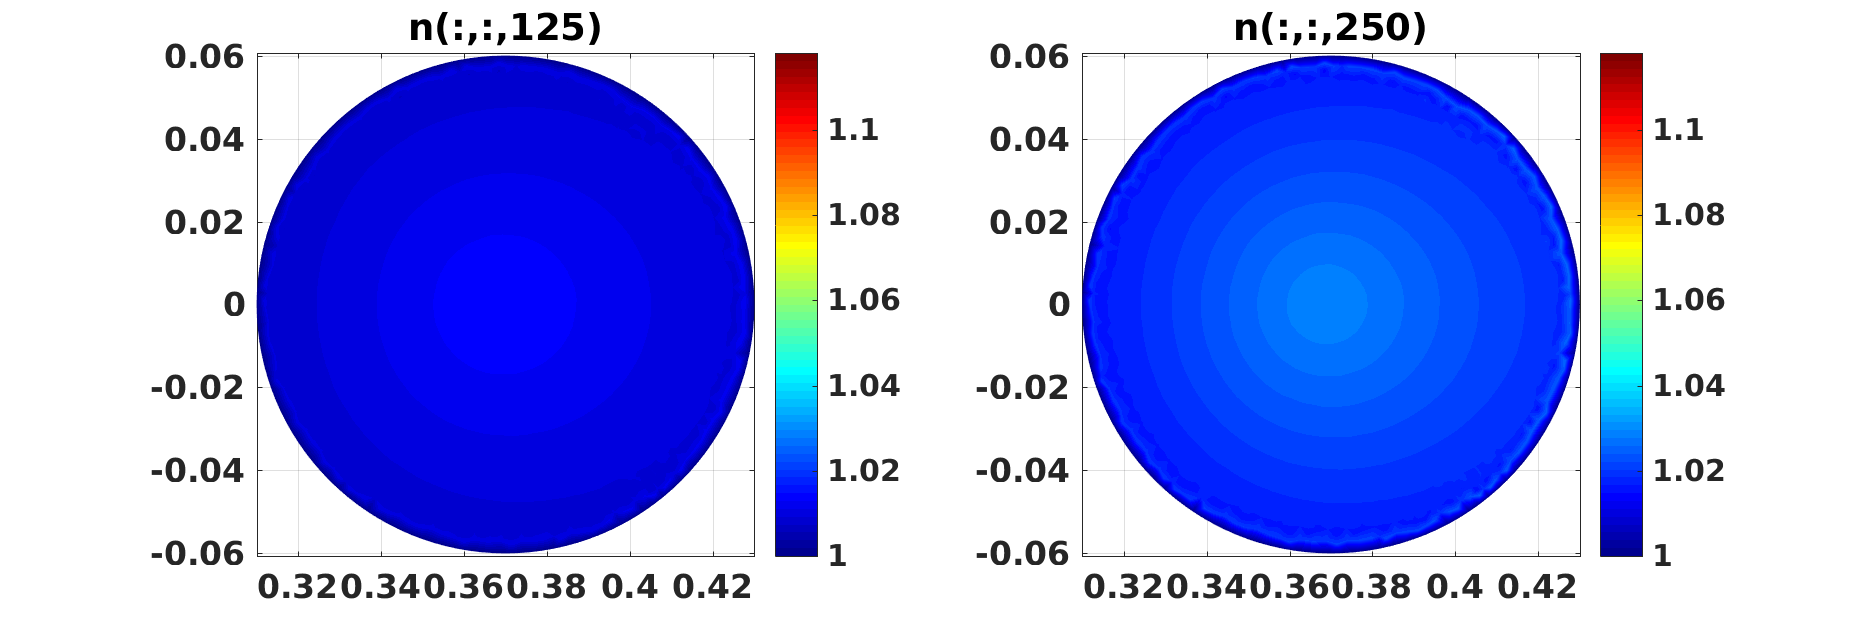
\includegraphics[scale=0.24]{../SImulacao_breakdown/PDE/ntod1B9.png}  
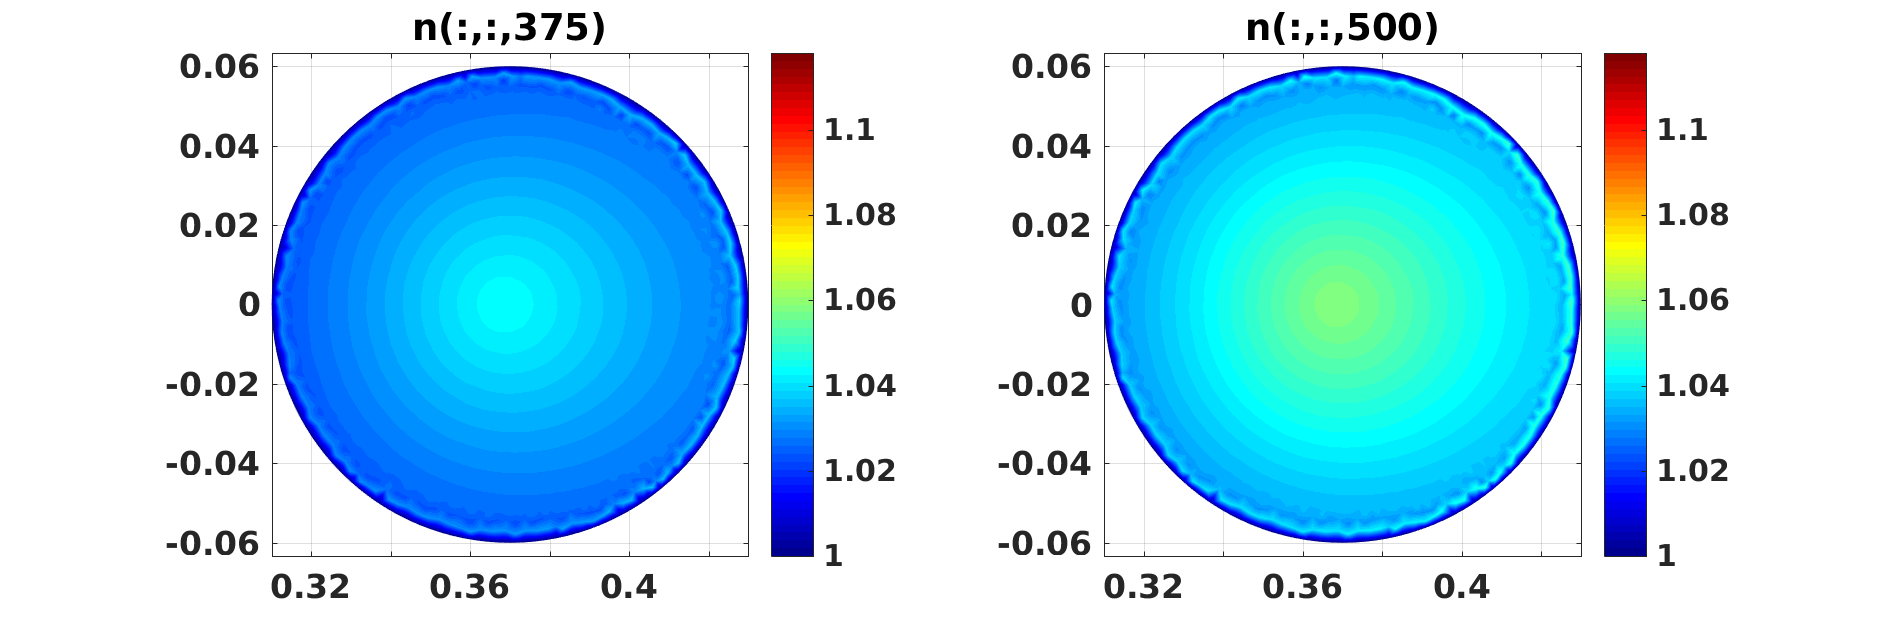
\includegraphics[scale=0.24]{../SImulacao_breakdown/PDE/ntod2B9.png}
\end{subfigure}
\begin{subfigure}{0.43\textwidth}
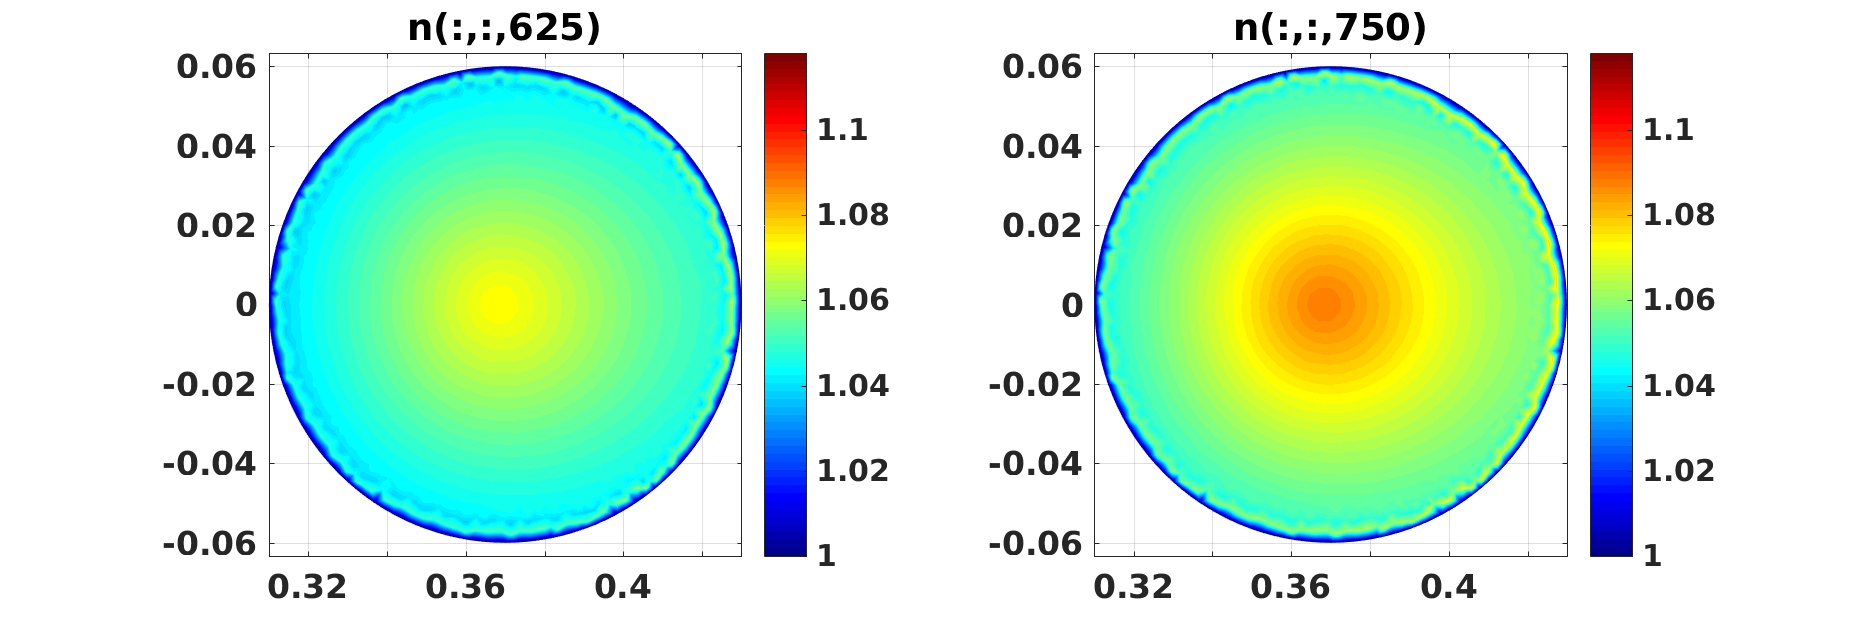
\includegraphics[scale=0.24]{../SImulacao_breakdown/PDE/ntod3B9.png} 
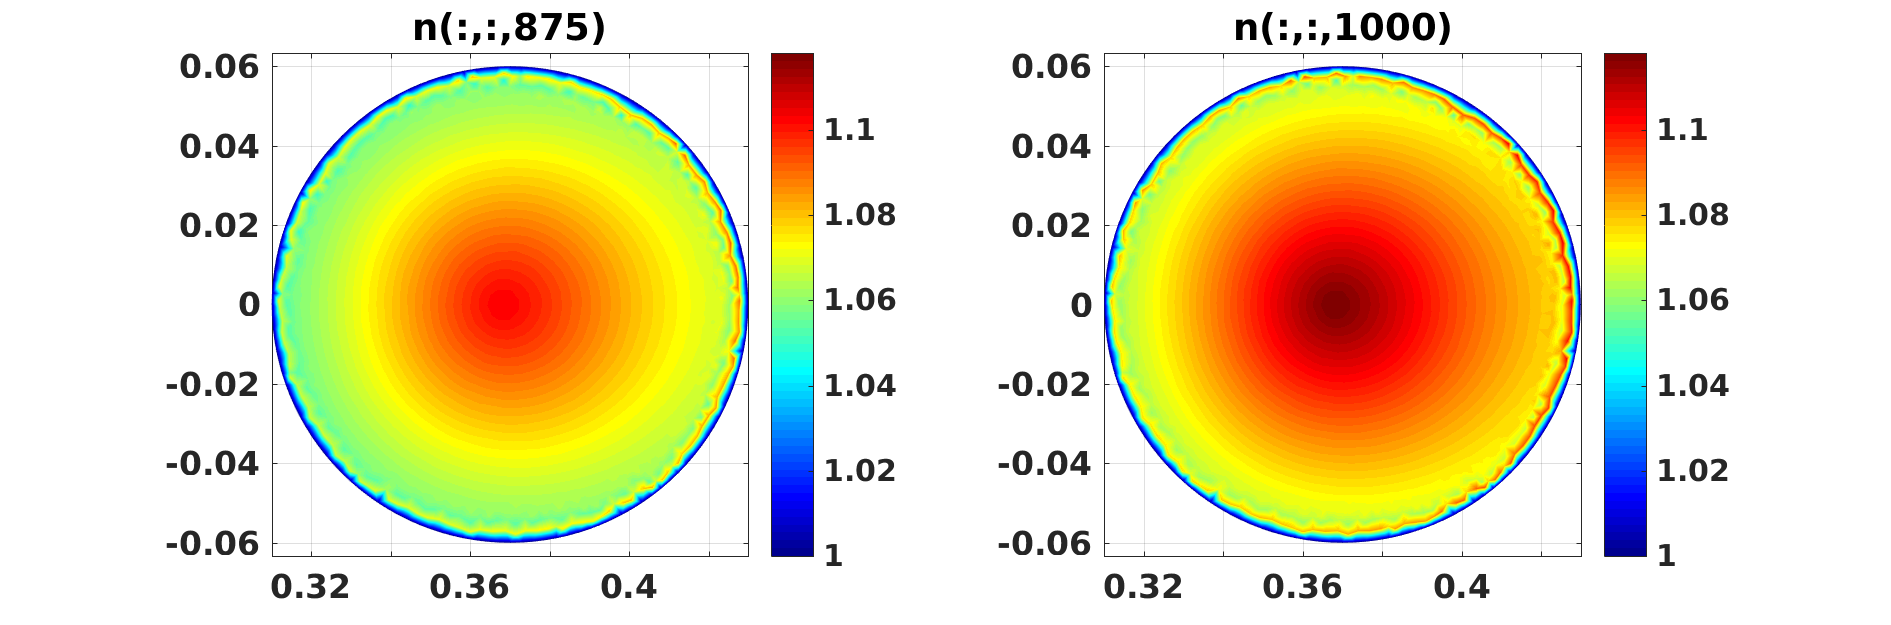
\includegraphics[scale=0.24]{../SImulacao_breakdown/PDE/ntod4B9.png} 
\end{subfigure}
\caption{Densidade de plasma ($m^{-3}$), fonte de partículas modelada através do modelo de Townsend ($dt=10^{-5}$\ s, $H_{max} = 0,003$ e $D=0,0002$\ $m^2s^{-1}$).}
\label{campplasmasil1}
\end{figure}
\end{frame}

\begin{frame}		
\frametitle{ Aproximação do campo magnético gerado pelo plasma}
\begin{figure}[H]
\begin{subfigure}{0.43\textwidth}
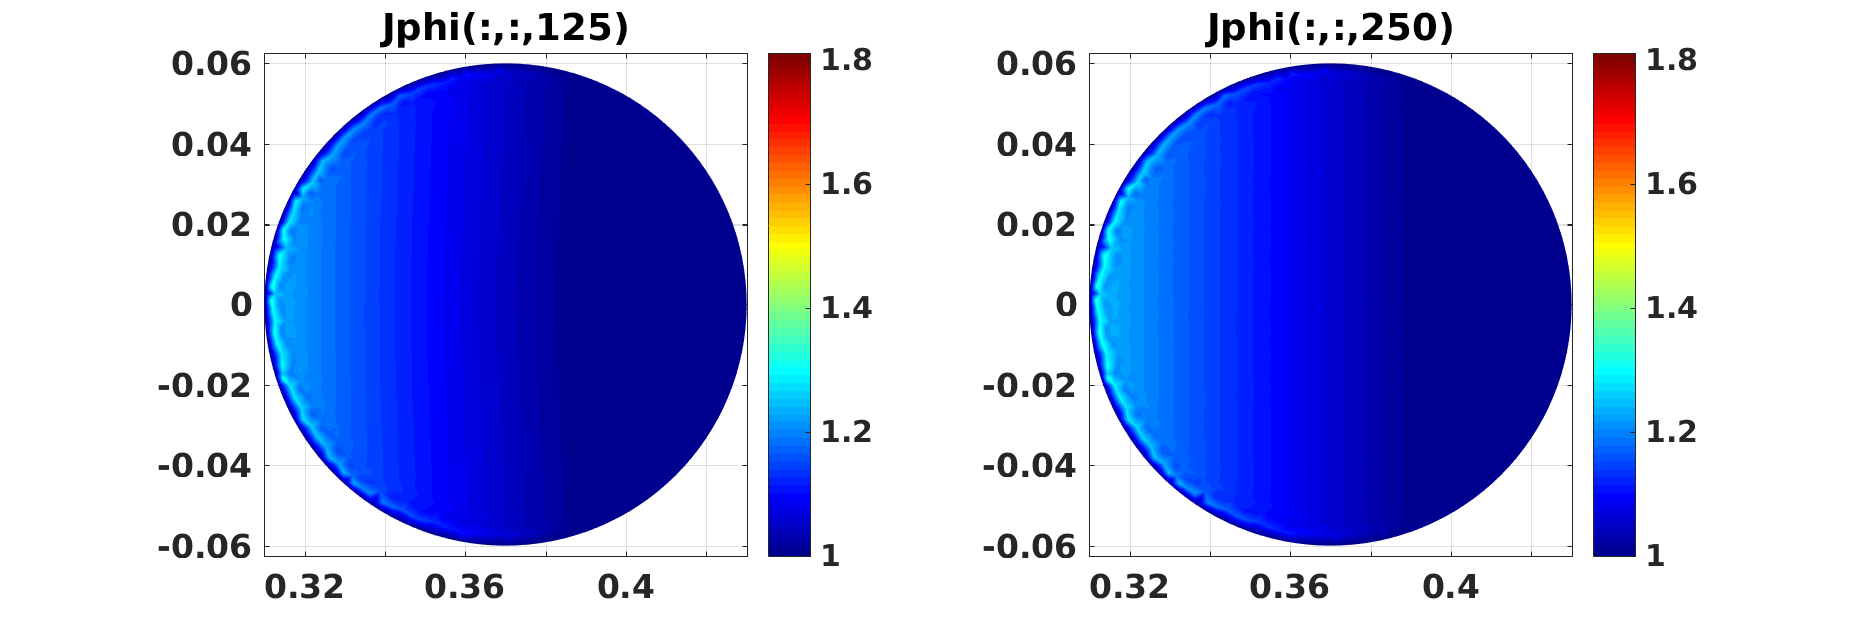
\includegraphics[scale=0.24]{../SImulacao_breakdown/PDE/Jphitod1B9.png}  
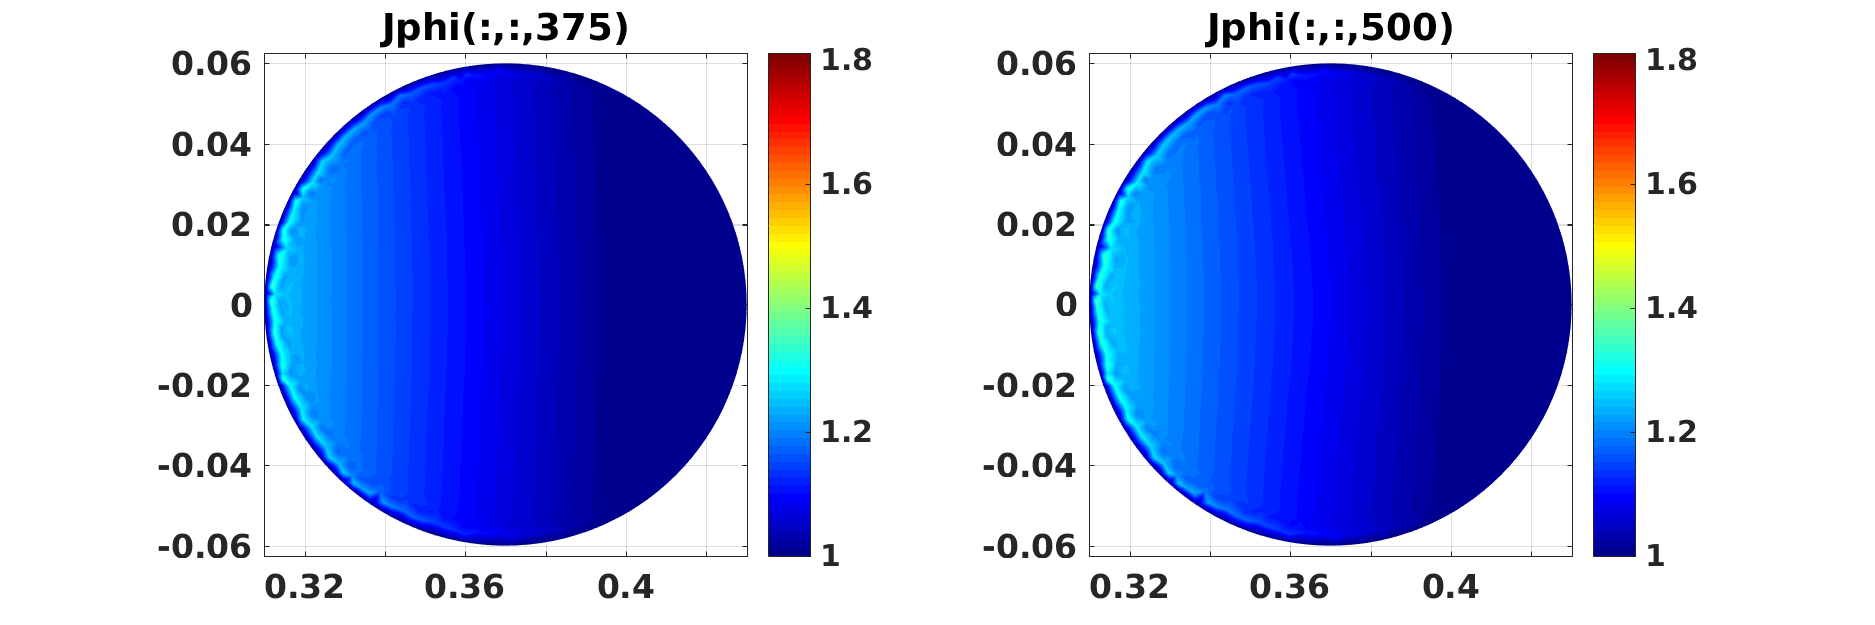
\includegraphics[scale=0.24]{../SImulacao_breakdown/PDE/Jphitod2B9.png}
\end{subfigure}
\begin{subfigure}{0.43\textwidth}
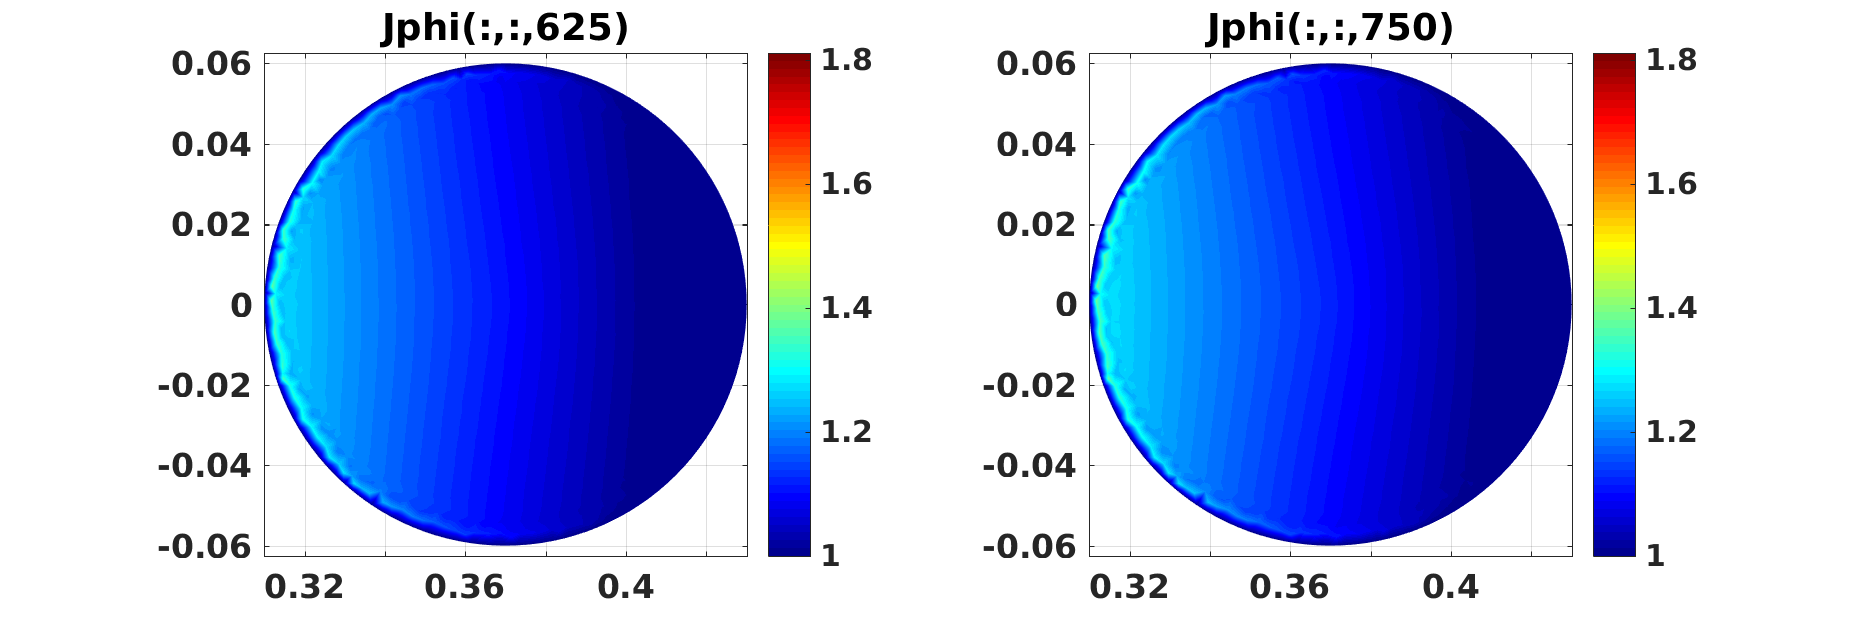
\includegraphics[scale=0.24]{../SImulacao_breakdown/PDE/Jphitod3B9.png} 
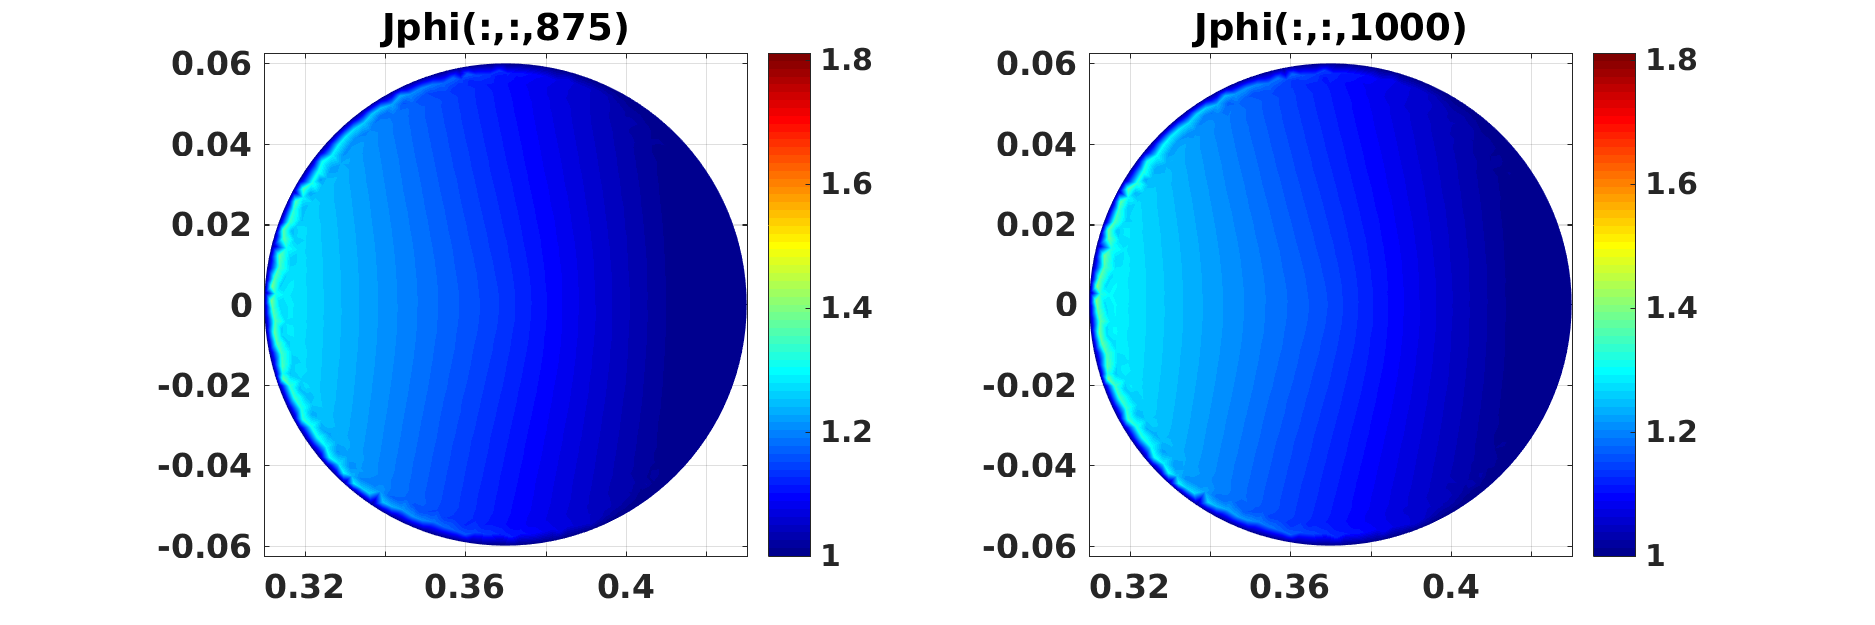
\includegraphics[scale=0.24]{../SImulacao_breakdown/PDE/Jphitod4B9.png} 
\end{subfigure}
\caption{Componente toroidal da densidade de corrente de plasma ($A/m^2$), fonte de partículas modelada através do modelo de Townsend ($dt=10^{-5}$\ s, $H_{max} = 0,003$ e $D=0,0002$\ $m^2s^{-1}$).}
\label{campplasmasil2}
\end{figure}
\end{frame}


\begin{frame}	
\frametitle{ Aproximação do campo magnético gerado pelo plasma}
\begin{figure}[H]
\begin{subfigure}{0.43\textwidth}
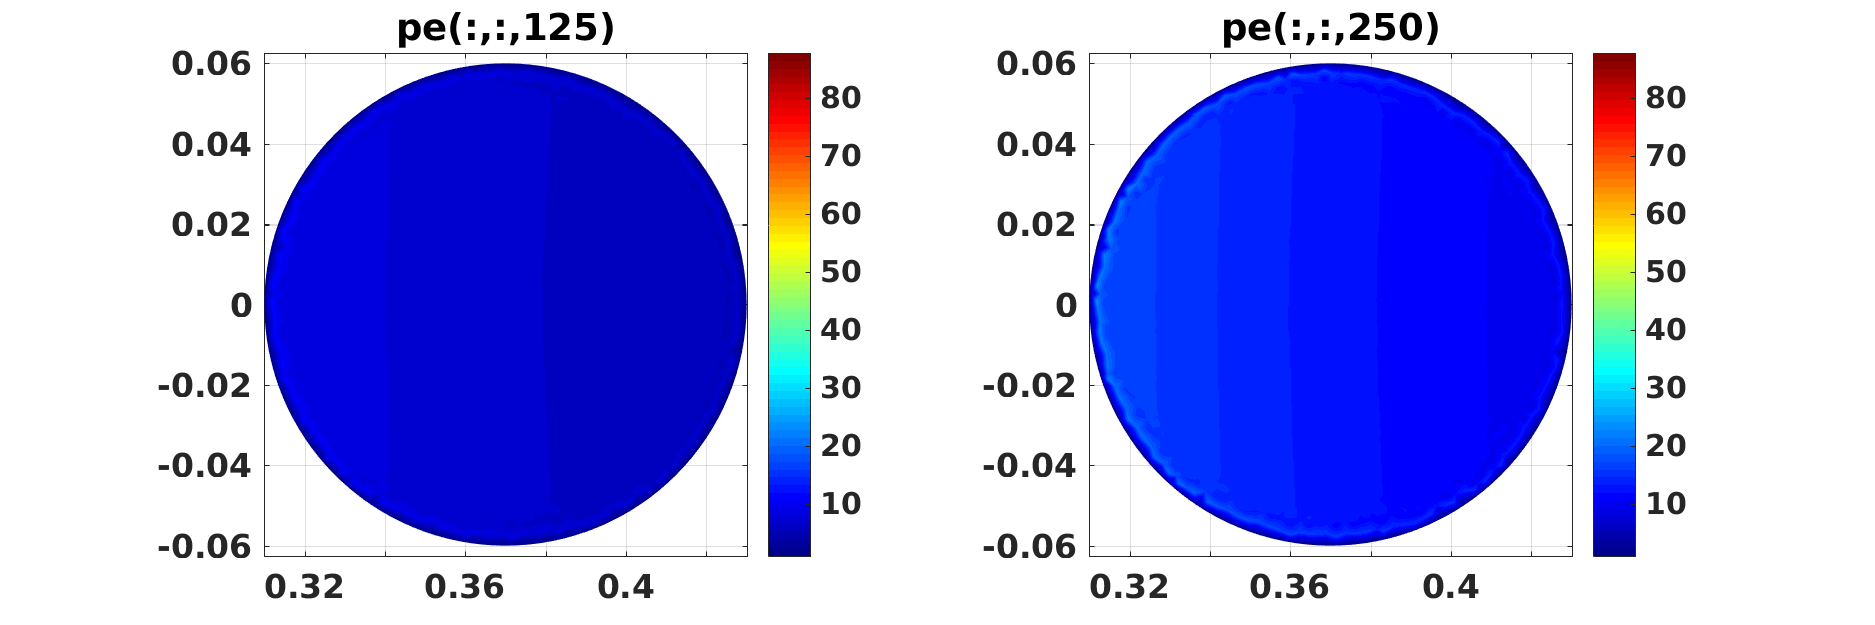
\includegraphics[scale=0.24]{../SImulacao_breakdown/PDE/petod1B9.png}  
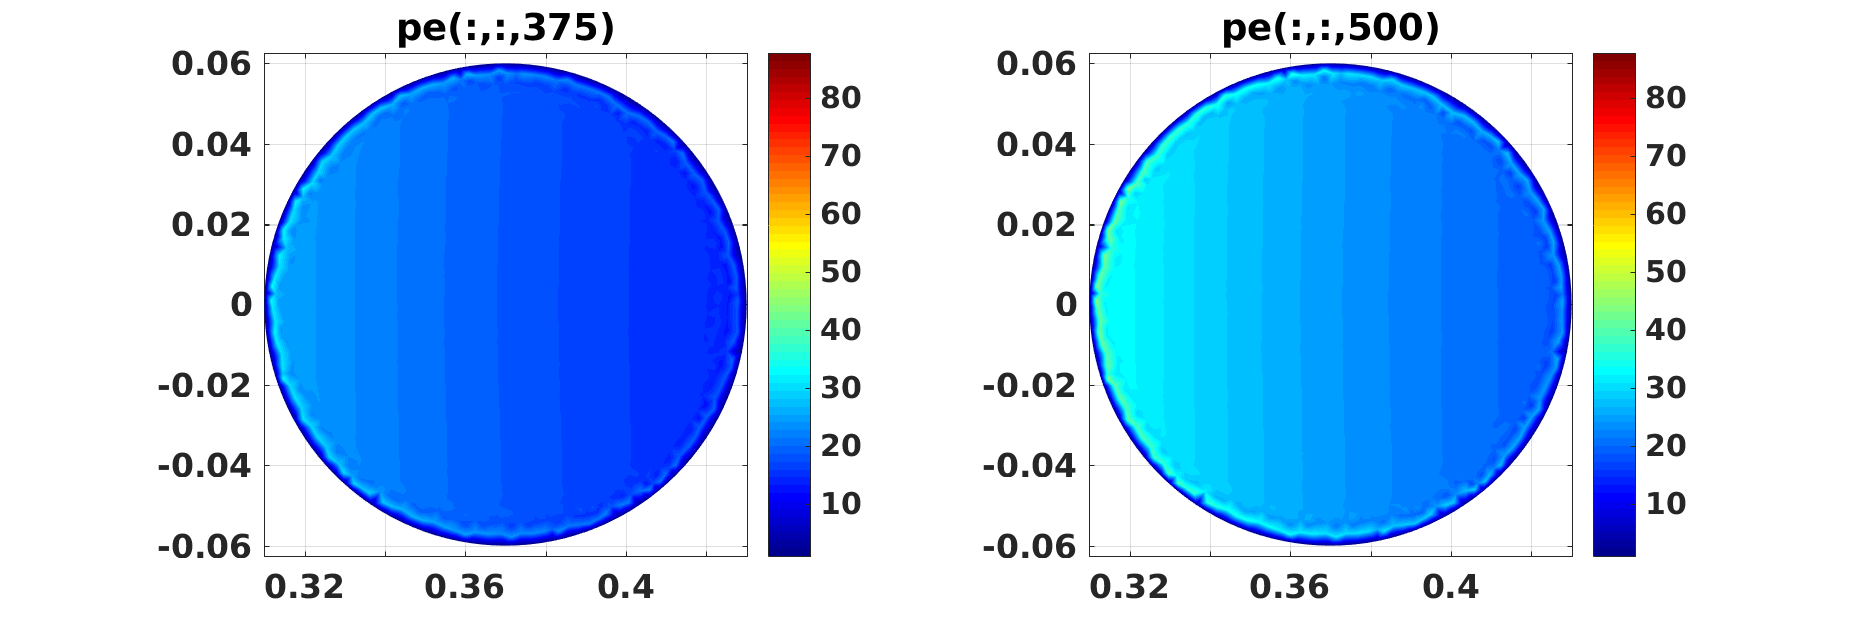
\includegraphics[scale=0.24]{../SImulacao_breakdown/PDE/petod2B9.png}
\end{subfigure}
\begin{subfigure}{0.43\textwidth}
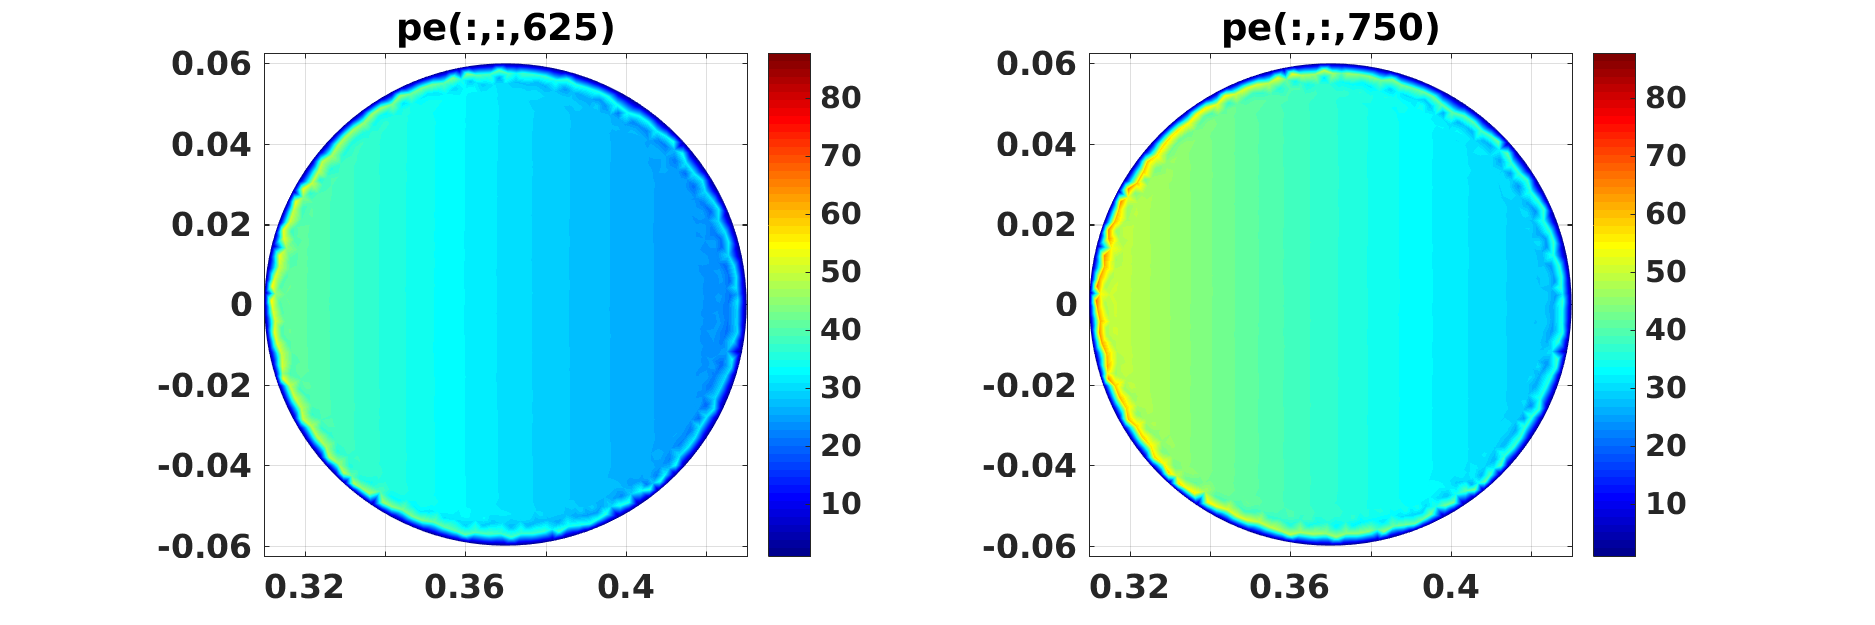
\includegraphics[scale=0.24]{../SImulacao_breakdown/PDE/petod3B9.png} 
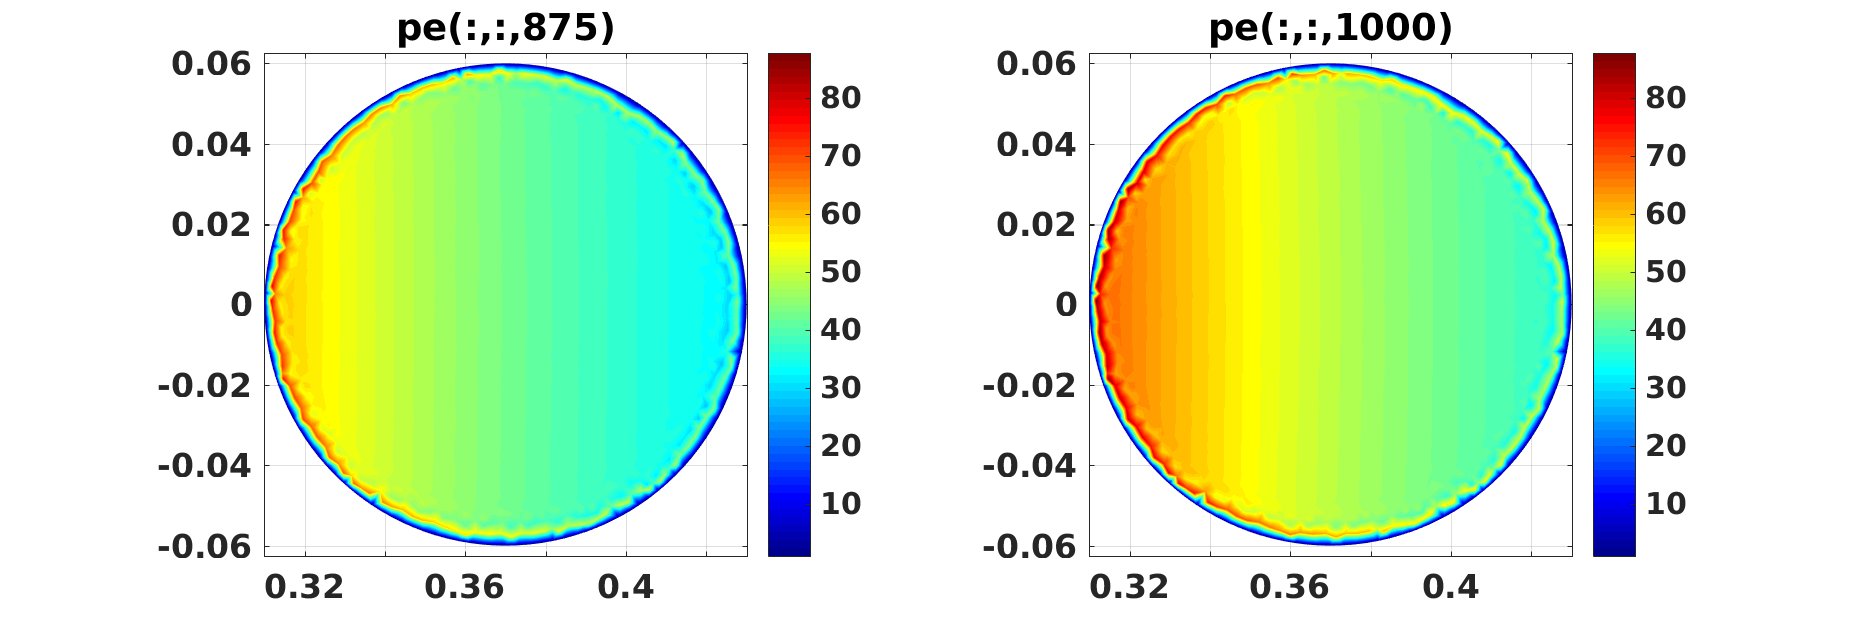
\includegraphics[scale=0.24]{../SImulacao_breakdown/PDE/petod4B9.png}
\end{subfigure}	
\caption{Pressão eletrônica ($Pa$), fonte de partículas modelada através do modelo de Townsend ($dt=10^{-5}$\ s, $H_{max} = 0,003$ e $D=0,0002$\ $m^2s^{-1}$).}
\label{campplasmasil3}
\end{figure}
\end{frame}


\begin{frame}		
\frametitle{ Aproximação do campo magnético gerado pelo plasma}
\begin{figure}[H]
\begin{subfigure}{0.43\textwidth}
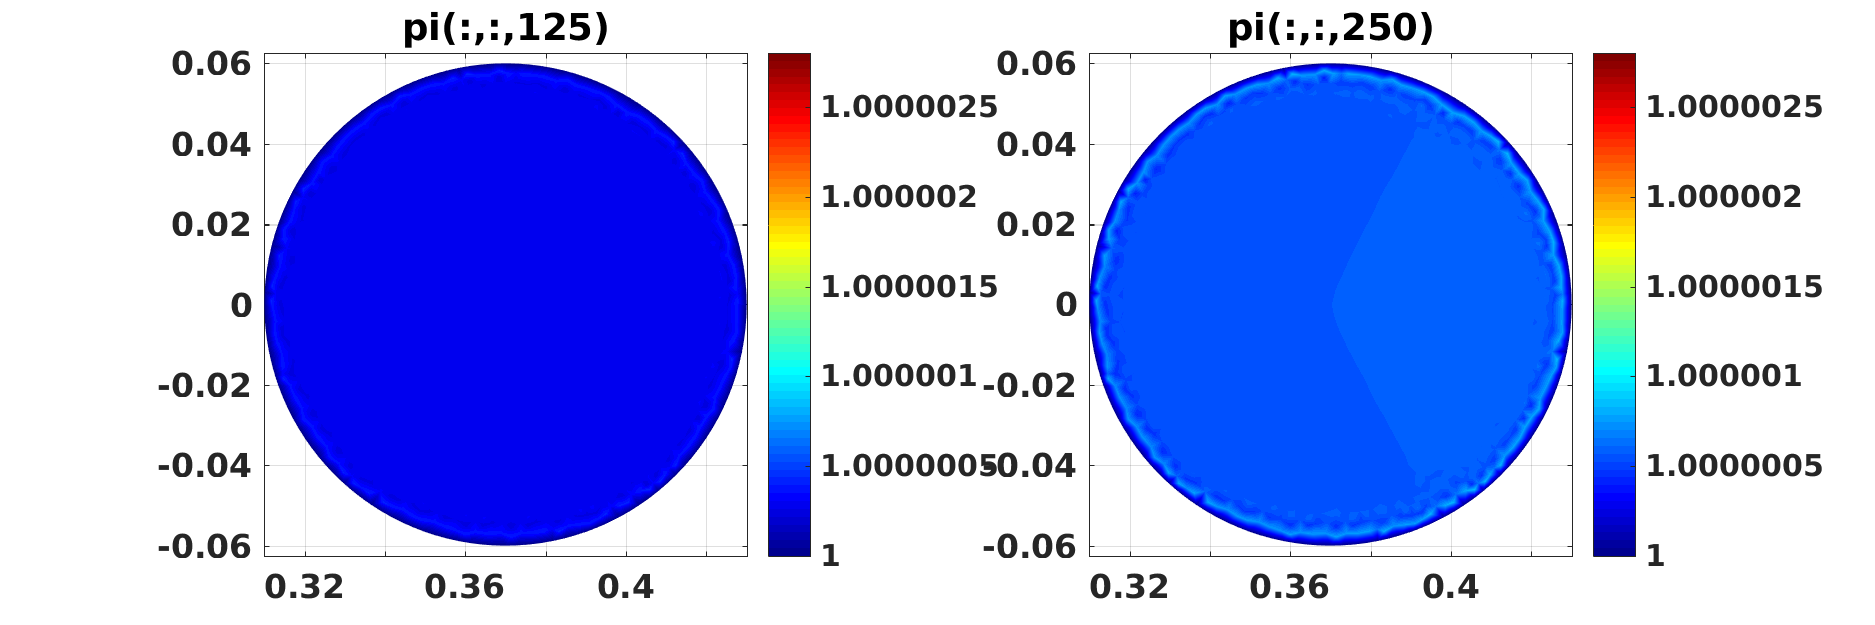
\includegraphics[scale=0.24]{../SImulacao_breakdown/PDE/pitod1B9.png}  
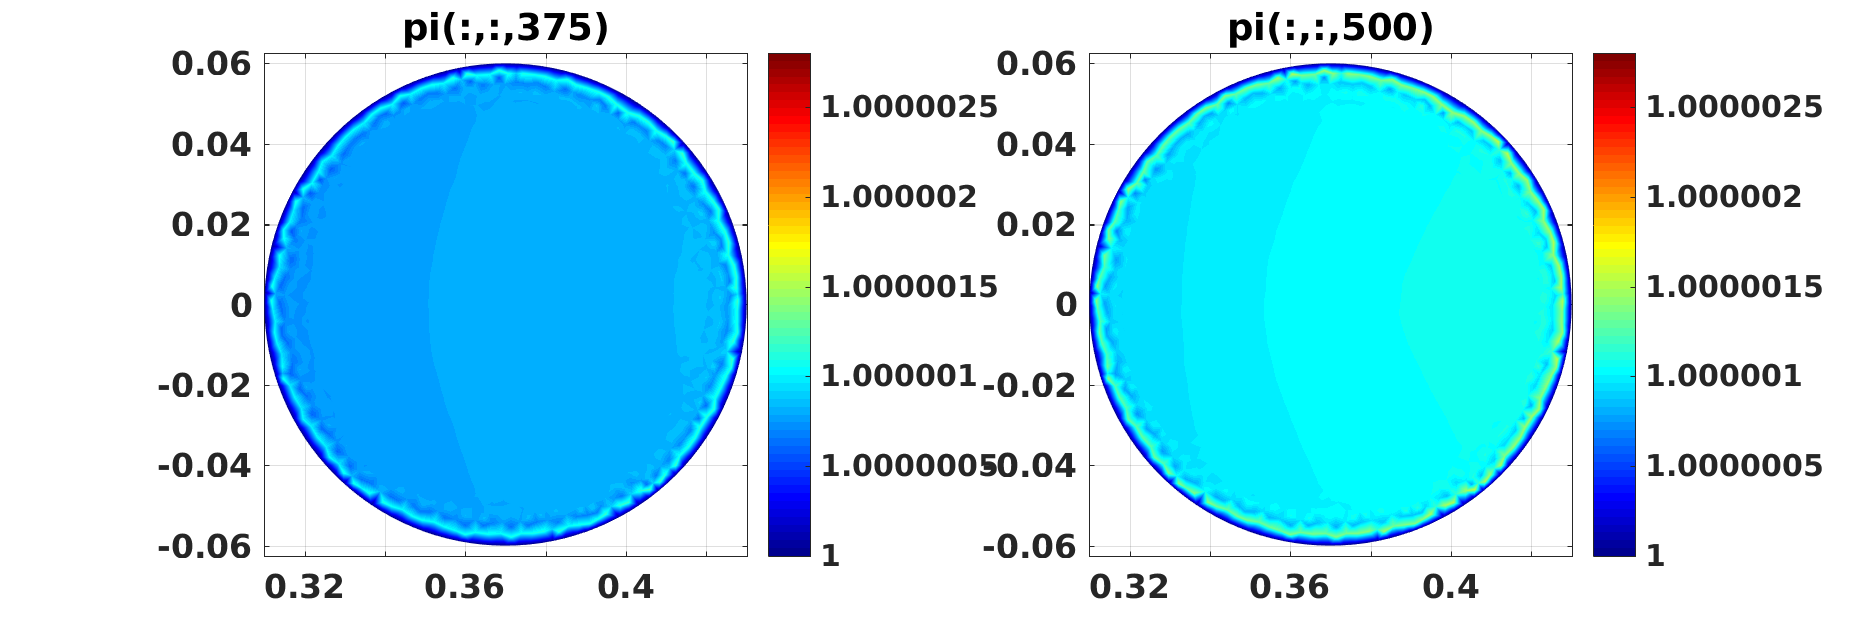
\includegraphics[scale=0.24]{../SImulacao_breakdown/PDE/pitod2B9.png} 
\end{subfigure}
\begin{subfigure}{0.43\textwidth}
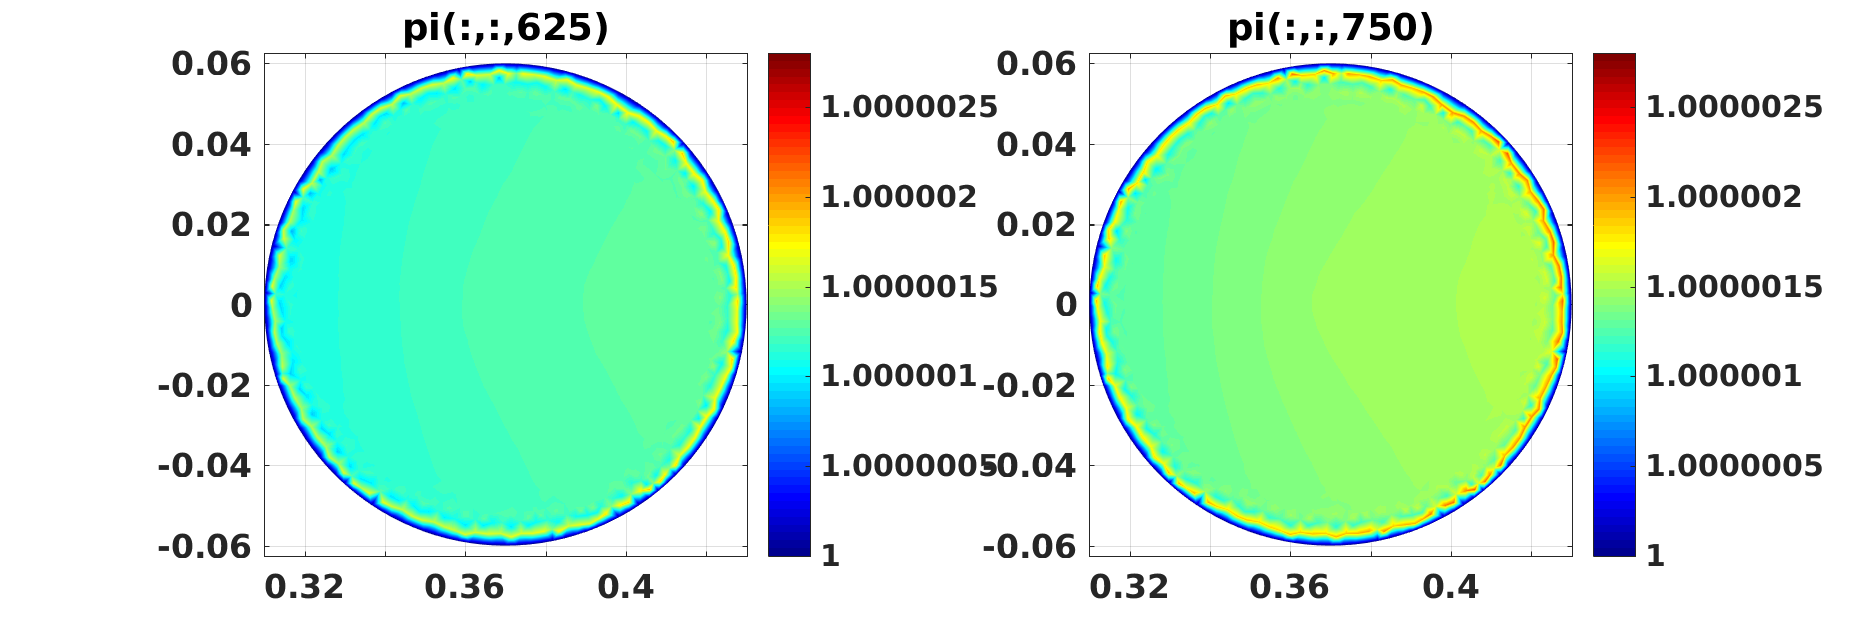
\includegraphics[scale=0.24]{../SImulacao_breakdown/PDE/pitod3B9.png} 
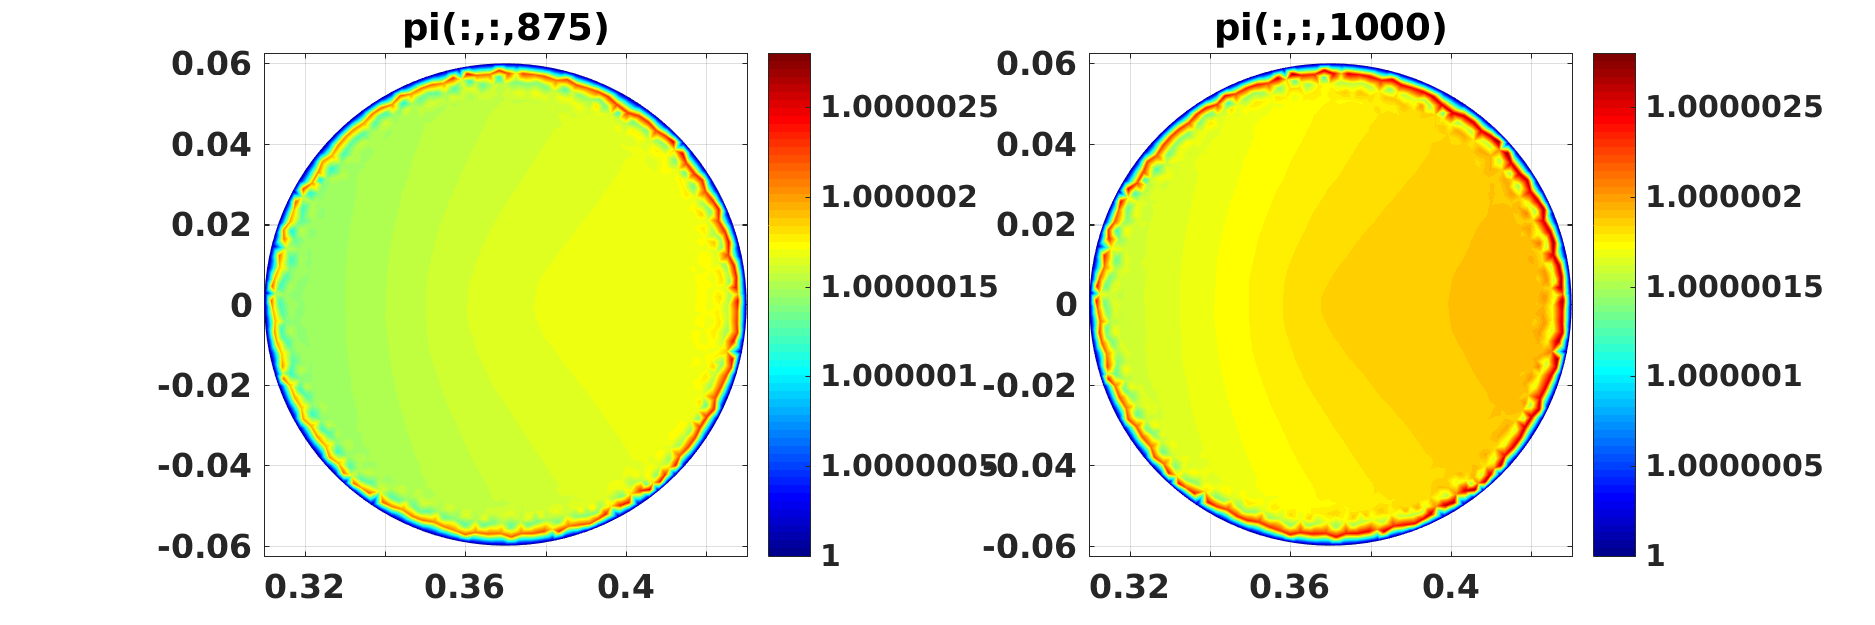
\includegraphics[scale=0.24]{../SImulacao_breakdown/PDE/pitod4B9.png} 
\end{subfigure}
\caption{Pressão iônica ($Pa$), aproximação da ionização por uma gaussiana ($dt=10^{-5}$\ s, $H_{max} = 0,003$ e $D=0,0002$\ $m^2s^{-1}$).}
\end{figure}

\begin{frame}		
\frametitle{Superfícies de fluxo magnético poloidal  }
\begin{itemize}
\item Multiplicando  cada tabela de Green por uma corrente, somando tudo e chamando a função \textit{contour} do MATLAB obtemos a figura \ref{fig: equipotenc} onde temos as superfícies de fluxo magnético poloidal gerado pelas bobinas. 

\item E se adicionarmos o campo gerado pela corrente de plasma obtemos a figura \ref{fig: equipotenc2} onde se encontram as superfícies de fluxo magnético poloidal gerado pelas bobinas mais o campo magnético gerado pela corrente de plasma. No caso o o campo magnético gerado pela corrente de plasma é simulado por 5 bobinas localizadas no centro da secção reta do tokamak NOVA-FURG.
\end{itemize}
\end{frame}
\begin{comment}
    \begin{frame}
		\frametitle{Sistema de equações}
\begin{equation}
\bm{\nabla} \cdot \bm{E}_{pl} = \frac{\rho}{\epsilon_0},
\end{equation}

\begin{equation}
\bm{\nabla} \times \bm{E}_{pl} = -\frac{\partial \bm{B}_{pl}}{\partial t},
\end{equation}

\begin{equation}
\bm{\nabla} \times \bm{B}_{pl} = \mu_0 (\bm{J} + \epsilon_0 \frac{\partial \bm{E}_{pl}}{\partial t} ),
\end{equation}

\begin{equation}
\rho(\bm{r},t) =   n(\bm{r},t)(q_e+q_i),
\end{equation}

\begin{equation}
\bm{J}(\bm{r},t) =  (q_e \bm{u}_e(\bm{r},t)+q_i \bm{u}_i(\bm{r},t)) n(\bm{r},t).  
\end{equation}
	\end{frame}	
\end{comment}

$\nu_{in} - \nu_{loss}$ 
\begin{comment}

\begin{figure}[H]
\begin{center}
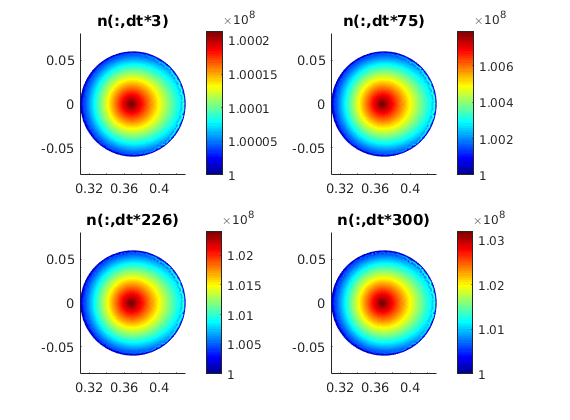
\includegraphics[scale=1]{../SImulacao_breakdown/PDE/nB.png} 
\caption{Densidade de partículas.}
\end{center}
\end{figure}
\begin{figure}[H]
\begin{center}
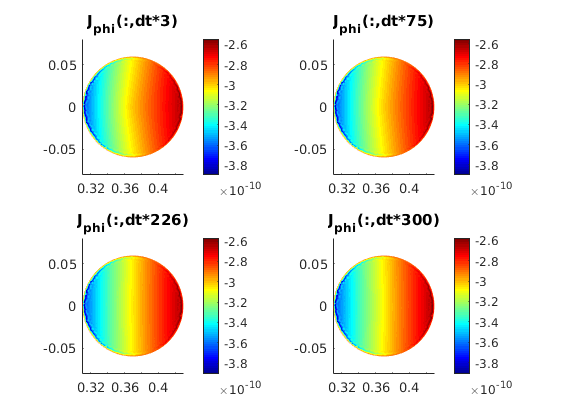
\includegraphics[scale=1]{../SImulacao_breakdown/PDE/JB.png} 
\end{center}
\caption{Densidade de corrente toroidal.}
\label{densidadeB}
\end{figure}
\begin{figure}[H]
\begin{center}
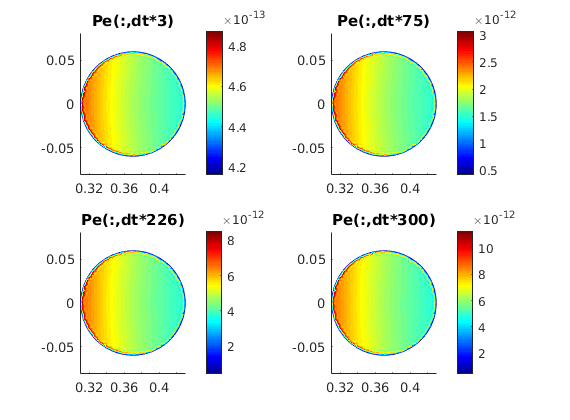
\includegraphics[scale=1]{../SImulacao_breakdown/PDE/peB.png} 
\caption{Pressão eletrônica.}
\end{center}
\end{figure}
\begin{figure}[H]
\begin{center}
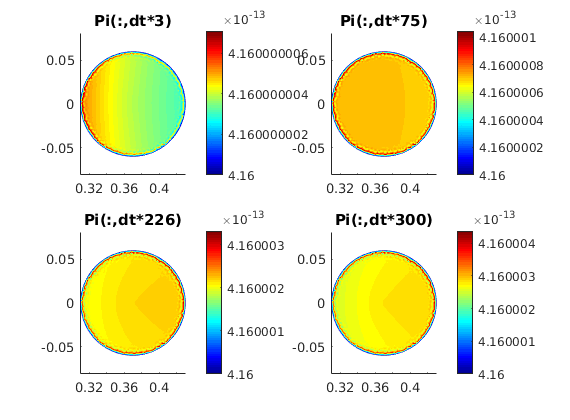
\includegraphics[scale=1]{../SImulacao_breakdown/PDE/piB.png} 
\end{center}
\caption{Pressão iônica.}
\label{pressaoB}
\end{figure}

\begin{figure}[H]
\begin{center}
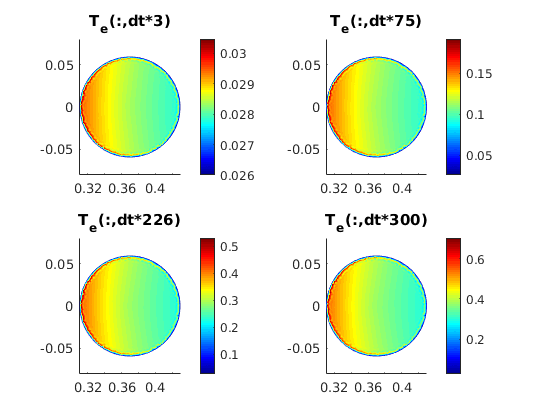
\includegraphics[scale=1]{../SImulacao_breakdown/PDE/TeB.png} 
\caption{Temperatura de elétrons.}
\end{center}
\end{figure}
\begin{figure}[H]
\begin{center}
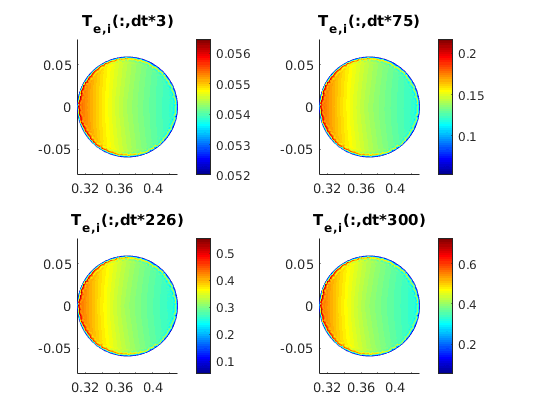
\includegraphics[scale=1]{../SImulacao_breakdown/PDE/TeiB.png} 
\end{center}
\caption{Temperatura de elétrons-íons.}
\label{temperaturaB}
\end{figure}

Agora rodando com o campo magnético gerado pelo plasmas sendo simulado por uma bobina no centro da câmera de vácuo. Dados $dt=1e-5$s, $n_0=1e8$, $ng = 0.05/1.38e-23/300$, $D=-0.002$, $T_{e_0} = 0.026$, Com todos os coeficientes de transporte implementados.
\begin{figure}[H]
\begin{center}
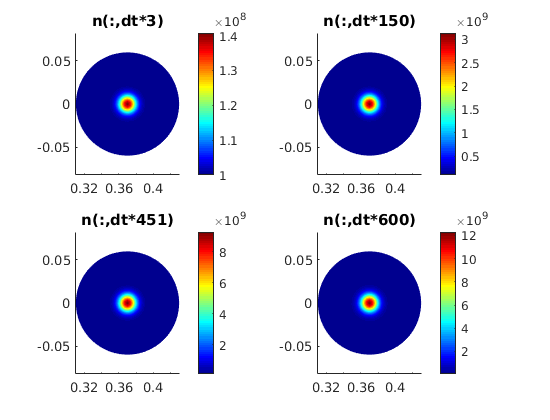
\includegraphics[scale=1]{../SImulacao_breakdown/PDE/nB2.png} 
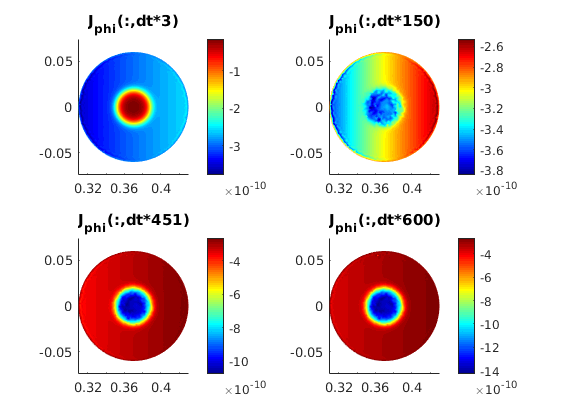
\includegraphics[scale=1]{../SImulacao_breakdown/PDE/JB2.png} 
\end{center}
\caption{Densidade de partículas e densidade de corrente toroidal.}
\label{densidadeB}
\end{figure}
\begin{figure}[H]
\begin{center}
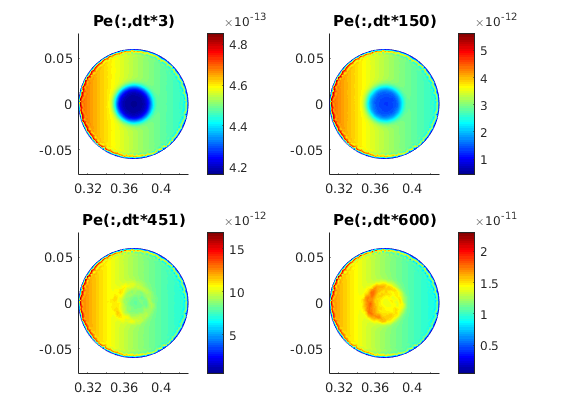
\includegraphics[scale=1]{../SImulacao_breakdown/PDE/peB2.png} 
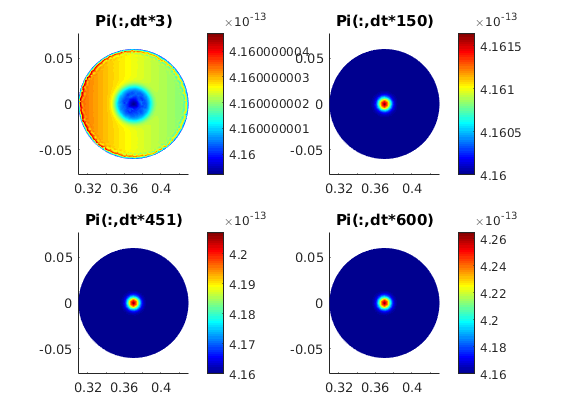
\includegraphics[scale=1]{../SImulacao_breakdown/PDE/piB2.png} 
\end{center}
\caption{Pressões eletrônica e iônica.}
\label{pressaoB}
\end{figure}

\begin{figure}[H]
\begin{center}
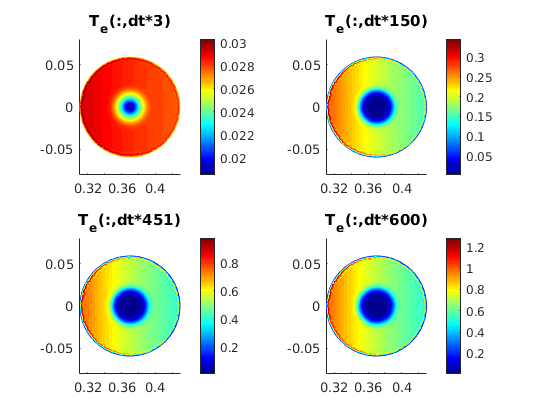
\includegraphics[scale=1]{../SImulacao_breakdown/PDE/TeB2.png} 
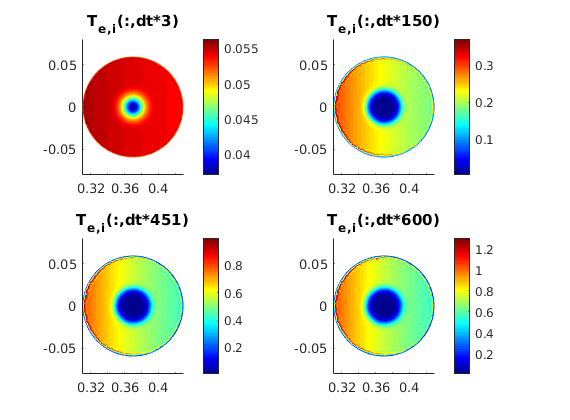
\includegraphics[scale=1]{../SImulacao_breakdown/PDE/TeiB2.png} 
\end{center}
\caption{Temperatura elétrons e elétrons-íons.}
\label{temperaturaB}
\end{figure}
\end{comment}

\begin{comment}
\begin{figure}[H]
\begin{center}
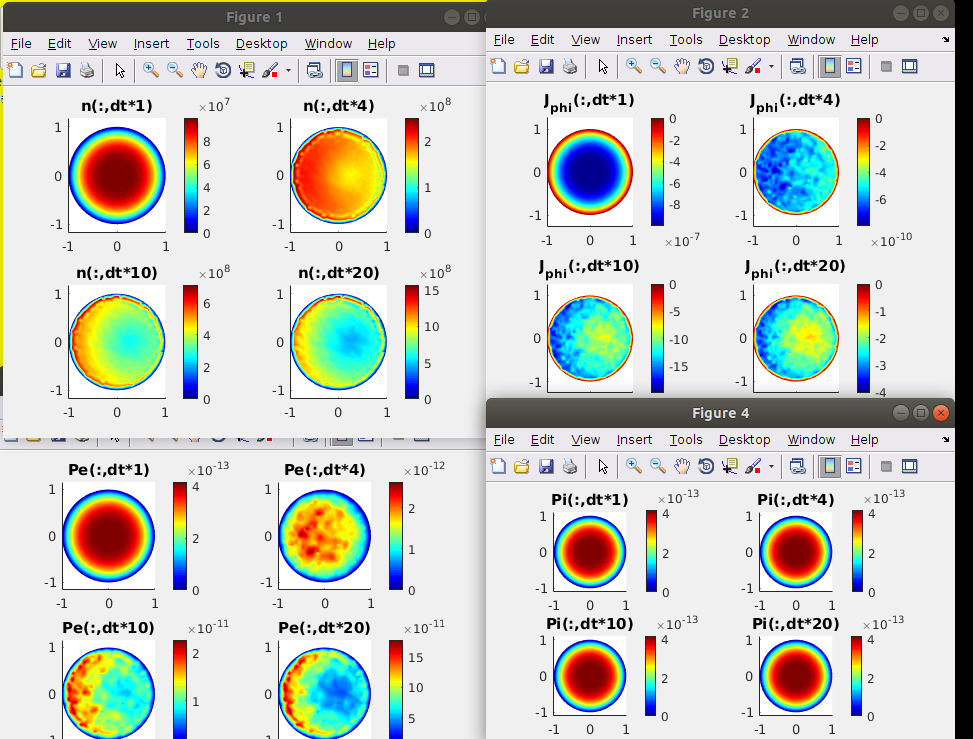
\includegraphics[scale=0.4]{../SImulacao_breakdown/PDE/hmas01-4eqs.png} 
\end{center}
\caption{Simulação do sistema com $dt=1e-4$s, $n_0=1e8$, $ng = 0.05/1.38e-23/300$, $D=0.15$, $x_0=0.25$, $s_0=1$ e $\sigma=1$ e $T_{e_0} = 0.026$.}
\end{figure}


O resultado obtido rodando a rotina principal, código \ref{codigos7}, foi a Figura \ref{fig: densgaussiana}, onde o sistema está com $dt=1e-5$s, $n_0=1e8$, $ng = 0.05/1.38e-23/300$, $D=-0.002$, $T_{e_0} = 0.026$. 
\begin{figure}[H]
\label{fig: densgaussiana}
\begin{center}
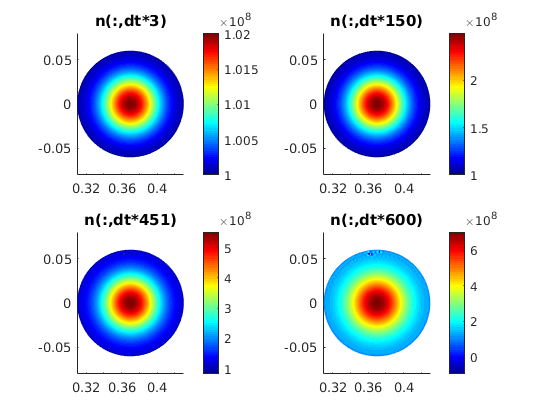
\includegraphics[scale=1]{../SImulacao_breakdown/PDE/nG.png} 
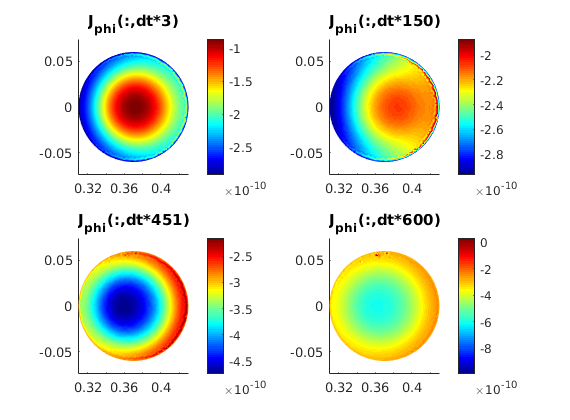
\includegraphics[scale=1]{../SImulacao_breakdown/PDE/JG.png} 
\end{center}
\caption{Densidade de partículas e densidade de corrente - Aproximação Gaussiana.}
\end{figure}
\begin{figure}[H]
\begin{center}
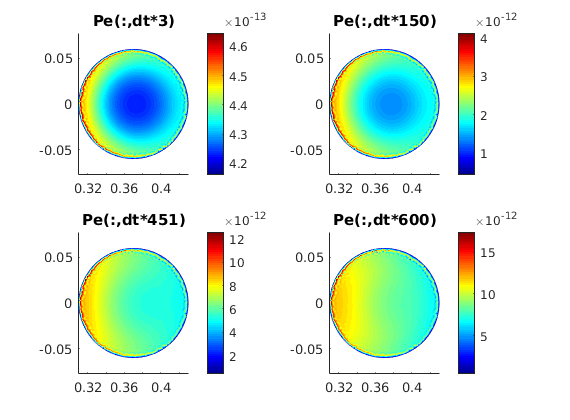
\includegraphics[scale=1]{../SImulacao_breakdown/PDE/peG.png} 
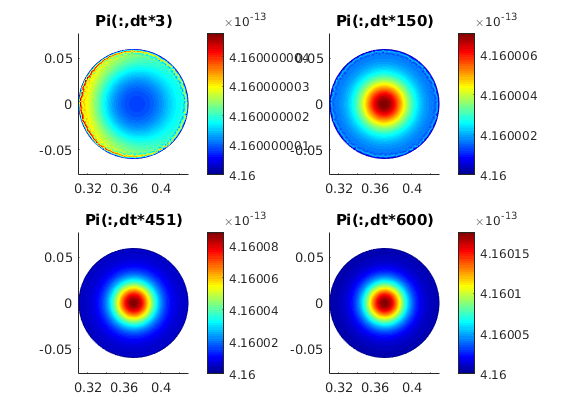
\includegraphics[scale=1]{../SImulacao_breakdown/PDE/piG.png} 
\end{center}
\caption{Pressões eletrônica e iônica - Aproximação Gaussiana.}
\end{figure}
\begin{figure}[H]
\begin{center}
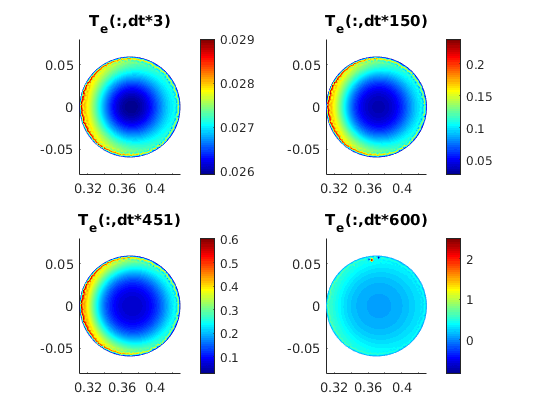
\includegraphics[scale=1]{../SImulacao_breakdown/PDE/TeG.png} 
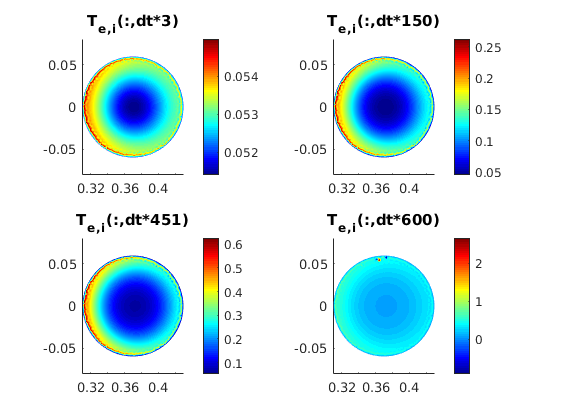
\includegraphics[scale=1]{../SImulacao_breakdown/PDE/TeiG.png} 
\end{center}
\caption{Temperatura elétrons e elétrons-íons - Aproximação Gaussiana.}
\end{figure}
E com uma malha mais refinada $H_{max}=0.002$ e desligando a fonte de partículas no tempo $25dt$, com os dados $dt=1e-8$s, $n_0=1e7$, $ng = 0.05/1.38e-23/300$, $D=-0.02$, $T_{e_0} = 0.026$, $s_0=10^{11}$, $x_0=0.015$ e $\sigma=0.00001$ .

\begin{figure}[H]
\label{fig: densgaussiana}
\begin{center}
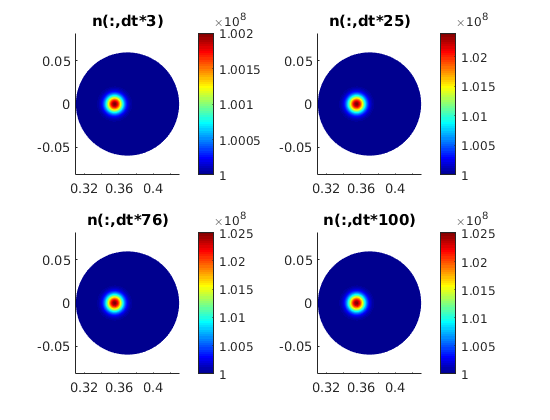
\includegraphics[scale=1]{../SImulacao_breakdown/PDE/nG2.png} 
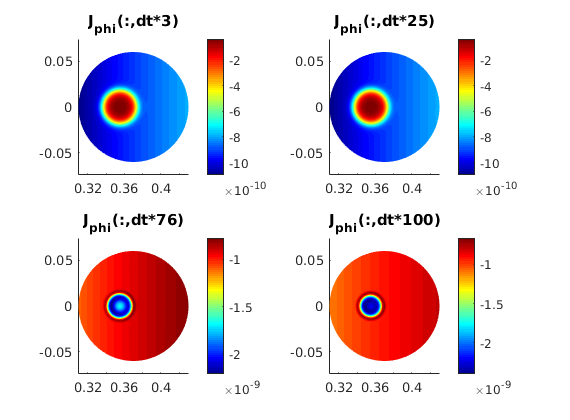
\includegraphics[scale=1]{../SImulacao_breakdown/PDE/JG2.png} 
\end{center}
\caption{Densidade de partículas e densidade de corrente - Aproximação Gaussiana.}
\end{figure}
\begin{figure}[H]
\begin{center}
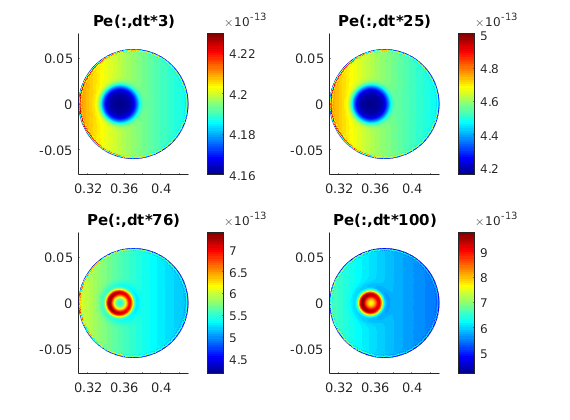
\includegraphics[scale=1]{../SImulacao_breakdown/PDE/peG2.png} 
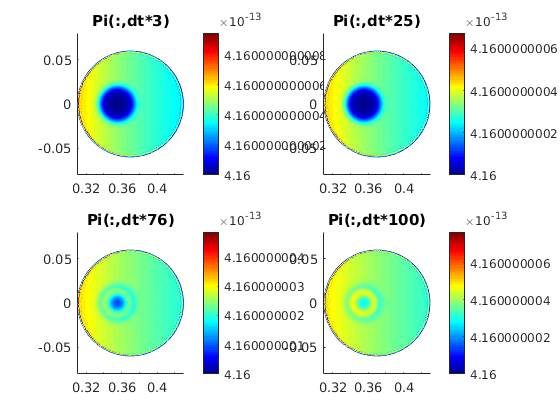
\includegraphics[scale=1]{../SImulacao_breakdown/PDE/piG2.png} 
\end{center}
\caption{Pressões eletrônica e iônica - Aproximação Gaussiana.}
\end{figure}
\end{comment}
\begin{equation}
\nabla^2 \bm{A}_{pl}=-\mu_0\bm{J} 
\end{equation}
\begin{equation}
\bm{B}_{pl} = \bm{\nabla} \times \bm{A}_{pl}
\end{equation}
\begin{equation}
\bm{E}_{pl}=-\frac{\partial \bm{A}_{pl}}{\partial t} .
\end{equation}
\begin{equation}
\bm{\nabla} \cdot \bm{E}_{pl} = \frac{\rho_{pl}}{\epsilon_0}=0,
\end{equation}
\begin{equation}
\bm{\nabla} \times \bm{E}_{pl} = -\frac{\partial \bm{B}_{pl}}{\partial t},
\end{equation}
\begin{equation}
\bm{\nabla} \times \bm{B}_{pl} = \mu_0 (\bm{J} + \epsilon_0 \frac{\partial \bm{E}_{pl}}{\partial t} ).
\end{equation}

\begin{comment}
Como condições de fronteira em coordenadas pseudo-toroidais para a densidade numérica $n(\bm{r},t)$ teremos $n(\bm{r},0)=n_0$ para todos os valores de $\bm{r}$. Definimos um $R_{mim}$ que será o menor valor da nossa malha e $n_0$  é o valor inicial da densidade numérica. 

%Para a densidade de corrente $\bm{J}(\bm{r},t)$ teremos $\bm{J}(\bm{r},0) = 0 \bm{r_0}+0 \bm{\theta_0}+ 0 \bm{\phi_0}=\bm{0}$ para todos os valores de $\bm{r}$.

Da condição inicial da densidade numérica tiramos a condição inicial para a densidade de carga através de $\rho(\bm{r},t) =   n(\bm{r},0)(q_e+q_i)$. O mesmo vale para a condição inicial da densidade de corrente $\bm{J}(\bm{r},0)=(q_e \bm{u}_e(\bm{r},0)+q_i \bm{u}_i(\bm{r},0)) n(\bm{r},0)$.

As condições iniciais para os campos eletromagnéticos $\bm{E}_{ext}$ e $\bm{B}_{ext}$ saem da distribuição de campos já calculadas. 

A condição inicial para a resistividade paralela de Sptizer $\eta$ é $\eta(\bm{r},0)=\eta_0$ para  $0 \leq \theta < 2 \pi$ e $ 0 \leq \phi < 2 \pi$ com $r=a_0$ e $r=R_{mim}$.

As condições iniciais para os escalares de pressão cinética $p_e$ e $p_i$ são $p_e(\bm{r},0)=p_{i0}$ e $p_e(\bm{r},0)=p_{e0}$ para $0 \leq \theta < 2 \pi$ e $ 0 \leq \phi < 2 \pi$ com $r=R_{mim}$. Para $r=a_0$ temos $p_e(\bm{r},0)=p_{i1}$ e $p_e(\bm{r},0)=p_{e1}$ para $0 \leq \theta < 2 \pi$ e $ 0 \leq \phi < 2 \pi$.

Temos as constantes $e$, $m_i$, $m_e$, $\epsilon_0$, $\mu_0$, $D$, $q_e$ e $q_i$. 
\end{comment}

\begin{comment}
Começando com os operadores $\nabla$ e $\nabla^2$, vamos escreve-los com as aproximações numéricas primeiro em coordenadas cartesianas
A densidade numérica no código é representada por uma matriz $n$, de $ng$ por $ng$ por $N_{time}$, onde $ng$ é o tamanho da malha para os valores de r e de z, e $N_{time}$ é o número de passos de tempo que será calculada a simulação. Ou seja temos $n(i,j,it)$ com $i$ e $j$ podendo variar entre $1$ e $ng$ e $it$ entre $1$ e $N_{time}$.

Temos então $\nabla$ em duas dimensões de espaço como $\nabla = \hat{e}_r \frac{\partial}{\partial r} + \hat{e}_z \frac{\partial}{\partial z}$ então $\nabla n(i,j,it)$ fica
\begin{equation*}
\nabla n(i,j,it+1) = \frac{n(i+1,j,it)-n(i-1,j,it)}{dr} + \frac{n(i,j+1,it)-n(i,j-1,it)}{dz}
\end{equation*}
E $\nabla^2 n(i,j,it)$ fica
\begin{equation*}
\nabla^2 n(i,j,it+1) =  \frac{n(i+1,j,it)-2n(i,j,it)+n(i-1,j,it)}{dr^2} + \frac{n(i,j+1,it)-2n(i,j,it)+n(i,j-1,it)}{dz^2}
\end{equation*}

Então a equação da continuidade de massa $\frac{\partial n}{\partial t} = \nu_{ion} - \nu_{loss}+D\nabla^2n + \bm{J} \cdot \nabla \frac{1}{e}$  fica


Onde 
$$\nabla^2n(:,:,it) = \left( \frac{n(i+1,j,it)-2n(i,j,it)+n(i-1,j,it)}{dr^2} + \frac{n(i,j+1,it)-2n(i,j,it)+n(i,j-1,it)}{dz^2}\right)$$
que deve ser calculada para cada combinação de $i$ e $j$, sendo que nas fronteiras devemos por as condições iniciais. Mas o laplaciano $\nabla^2n(:,:,it)$ pode ser resolvido numericamente com o comando del2(n(:,:,it),dr). O intervalo de tempo $dt= \frac{t_f-t_i}{N_{time}}= 10^{-5}$ segundos, como $t_i=0$ temos $t_f=dtN_{time}$
\end{comment}
Os operadores são
\begin{equation*}
\bm{\nabla} f = \frac{\partial f}{\partial r} \hat{e}_r +  \frac{1}{r} \frac{\partial f}{\partial \phi} \hat{e}_\phi + \frac{\partial f}{\partial z} \hat{e}_z,
\end{equation*}
\begin{equation*}
\bm{\nabla} \cdot \bm{F} = \frac{1}{r}  \frac{\partial }{\partial r} \Big( r F_r \Big)+ \frac{1}{r} \frac{\partial F_\phi}{\partial \phi} +  \frac{\partial F_z}{\partial z} ,
\end{equation*} 
\begin{equation*}
\bm{\nabla} \times \bm{F} =  \left[\frac{1}{r} \frac{\partial F_z}{\partial \phi} - \frac{\partial F_\phi}{\partial z} \right]  \hat{e}_r + \left[  \frac{\partial F_r}{\partial z} -  \frac{\partial F_z}{\partial r}  \right] \hat{e}_\phi + \left[ \frac{1}{r} \frac{\partial}{\partial r}\Big( r F_\phi \Big) - \frac{1}{r} \frac{\partial F_r}{\partial \phi}  \right] \hat{e}_z,
\end{equation*} 
\begin{equation*}
\nabla^2 f = \frac{\partial^2 f}{\partial r^2} + \frac{1}{r} \frac{\partial f}{\partial r} + \frac{1}{r^2} \frac{\partial^2 f}{\partial \phi^2}  + \frac{\partial^2 f}{\partial z^2} .
\end{equation*}
Expandindo os operadores diferenciais nas equações do plasma, $\phi$ é o ângulo na direção toroidal e nas direções poloidais temos $r$ sendo a direção radial e $z$ sendo a direção vertical.
\begin{equation}
\frac{\partial n}{\partial t} = \nu_{ion} - \nu_{loss}+D \left[  \frac{\partial^2 n}{\partial r^2} + \frac{1}{r} \frac{\partial n}{\partial r} + \frac{1}{r^2} \frac{\partial^2 n}{\partial \phi^2}  + \frac{\partial^2 n}{\partial z^2} \right] + 
\end{equation}
\begin{equation}
\frac{1}{e}  \left[ \frac{1}{r}  \frac{\partial }{\partial r}\Big(r J_r\Big) + \frac{1}{r} \frac{\partial J_\phi}{\partial \phi} +  \frac{\partial J_z}{\partial z} \right] .
\end{equation}
Como $\bm{J}_r$ e $\bm{J}_z$ são assumidos nulos, e como assumimos simetria azimutal temos $\frac{\partial \bm{J}_\phi}{\partial \phi} = 0$ e $ \frac{1}{r^2} \frac{\partial^2 n}{\partial \phi^2}=0$ então o termo todo $\frac{1}{e} \bm{\nabla} \cdot \bm{J}$ desaparece e ficamos com
\begin{equation}
\frac{\partial n}{\partial t} = \nu_{ion} - \nu_{loss}+D \left[  \frac{\partial^2 n}{\partial r^2} + \frac{1}{r} \frac{\partial n}{\partial r}  + \frac{\partial^2 n}{\partial z^2} \right] .
\end{equation}
A equação de conservação do momento eletrônico, usando a simetria  $\frac{1}{r} \frac{\partial p_e}{\partial \phi}  = 0$ fica
\begin{equation}
\label{momenteletrico1} 
\frac{\partial \bm{J}}{\partial t} =  \frac{ne^2}{m_e} \bm{E} -\bm{J}(\nu_{in}+\nu_{en}+\nu_{ion}-\nu_{loss}) -\frac{e}{m_e}\bm{J} \times \bm{B}+\frac{e}{m_e} \left[ \frac{\partial p_e}{\partial r} \hat{e}_r + \frac{\partial p_e}{\partial z} \hat{e}_z \right] .
\end{equation}
E as equações para os campos gerados pelo plasma, lembrando que $\frac{\partial \bm{B}_{pl_r,\phi,z}}{\partial \phi} = \frac{\partial \bm{E}_{pl_r,\phi,z}}{\partial \phi} = 0$ ficam
\begin{equation}
\frac{1}{r}  \frac{\partial}{\partial r} \big( r E_{pl_r} \big) +  \frac{\partial E_{pl_z}}{\partial z}   = \frac{r}{\epsilon_0},
\end{equation}
\begin{equation}
\left[- \frac{\partial E_{pl_\phi}}{\partial z} \right]  \hat{e}_r + \left[  \frac{\partial E_{pl_r}}{\partial z} -  \frac{\partial E_{pl_z}}{\partial r}  \right] \hat{e}_\phi + \left[ \frac{1}{r} \frac{\partial}{\partial r} \big( r E_{pl_\phi} \big)  \right] \hat{e}_z = -\frac{\partial \bm{B}_{pl}}{\partial t},
\end{equation}
\begin{equation}
\left[ - \frac{\partial B_{pl_\phi}}{\partial z} \right]  \hat{e}_r + \left[  \frac{\partial B_{pl_r}}{\partial z} -  \frac{\partial B_{pl_z}}{\partial r}  \right] \hat{e}_\phi + \left[ \frac{1}{r} \frac{\partial}{\partial r} \big( r B_{pl_\phi} \big) \right] \hat{e}_z = \mu_0 (\bm{J} + \epsilon_0 \frac{\partial \bm{E}_{pl}}{\partial t} ) .
\end{equation}
O sistema que sera implementado é
\begin{equation}
\label{contfinal} 
\frac{\partial n}{\partial t} = \nu_{ion} - \nu_{loss}+D \left[  \frac{\partial^2 n}{\partial r^2} + \frac{1}{r} \frac{\partial n}{\partial r}  + \frac{\partial^2 n}{\partial z^2} \right] ,
\end{equation}
\begin{equation}
\frac{\partial \bm{J}}{\partial t} =  \frac{ne^2}{m_e} \bm{E} -\bm{J}(\nu_{in}+\nu_{en}+\nu_{ion}-\nu_{loss}) -\frac{e}{m_e}\bm{J} \times \bm{B}+\frac{e}{m_e} \left[ \frac{\partial p_e}{\partial r} \hat{e}_r + \frac{\partial p_e}{\partial z} \hat{e}_z \right],
\end{equation}
\begin{equation}
\frac{\partial p_e}{\partial t} = \frac{3}{2}(1+\frac{2 \nu_{en} + \nu_{ion} - \nu_{loss}}{2\nu_{ei}})\eta J^2  -\frac{2ne^2}{m_i} \eta (p_e-p_i),
\end{equation}
\begin{equation}
\frac{\partial p_e}{\partial t} = \frac{2ne^2}{m_i}\eta(p_e-p_i) .
\end{equation}


\begin{comment}
\begin{comment}
\begin{figure}[H]
\label{simul17}
\begin{center}
\includegraphics[scale=0.5]{../SImulacao_breakdown/Adaptacao_nova/Jphi(:,:,403).png}  
\caption{Resultado inicial, \textit{contourf} densidade numérica e densidade de corrente na direção toroidal, $dt=10e-5$s, $Ng = 65$.}
\end{center}
\end{figure}
\begin{figure}[H]
\label{simul18}
\begin{center}
\includegraphics[scale=0.5]{../SImulacao_breakdown/Adaptacao_nova/pion(:,:,403).png}  
\caption{Resultado inicial, \textit{contourf} pressões eletrônica e iônica, $dt=10e-6$s, $Ng = 65$.}
\end{center}
\end{figure}
\end{comment}
Alguns resultados iniciais usando o código \ref{codigos1} e considerando nulos os campos internos elétricos e magnéticos. Todos os tempos de cada variáveis macroscópicas em uma página.Ionização elétron-íon menos perda aproximada pela Gaussiana.
\begin{figure}[H]
\label{simul201}
\begin{center}
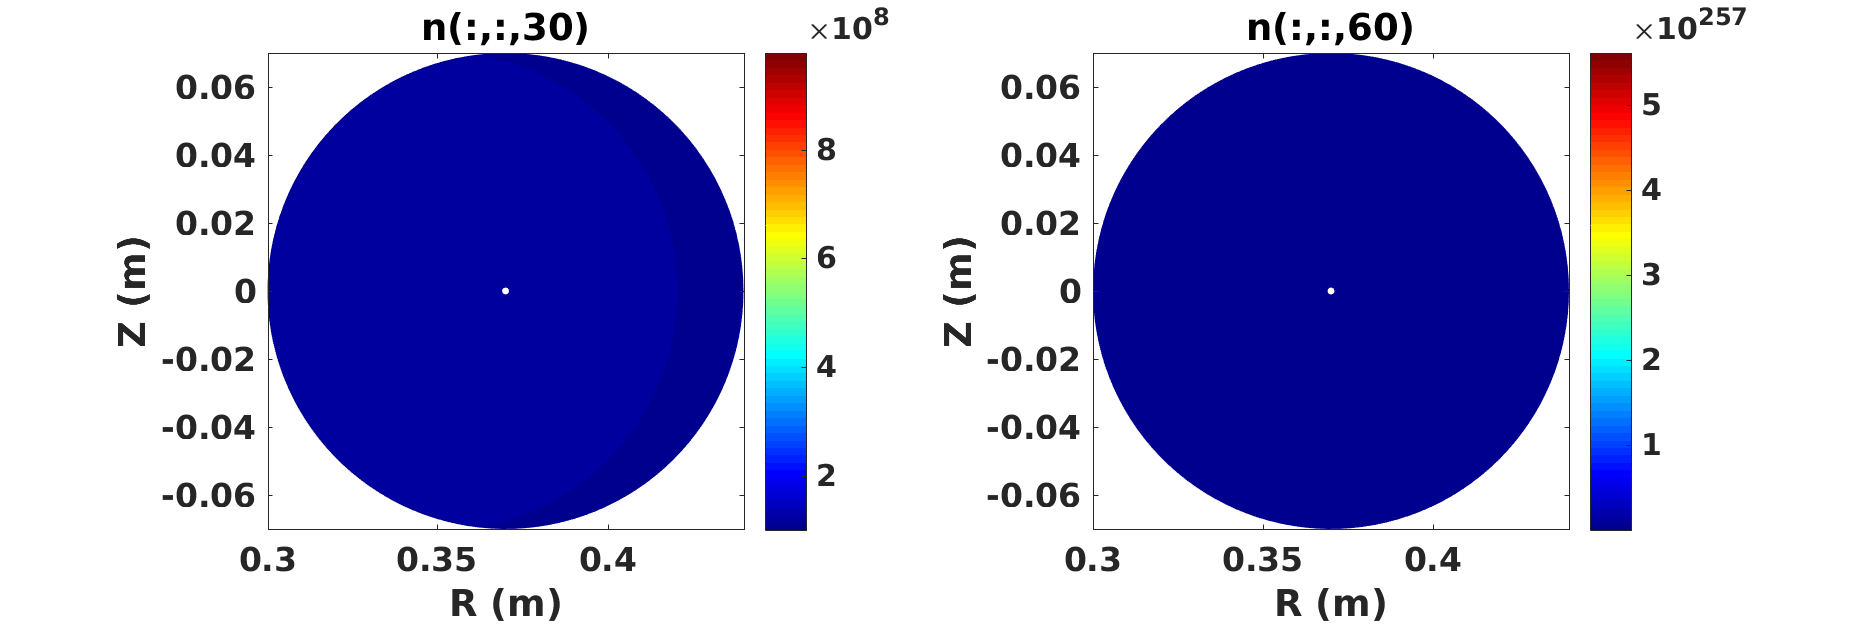
\includegraphics[scale=0.5]{../SImulacao_breakdown/Adaptacao_nova/ntod1.png}  
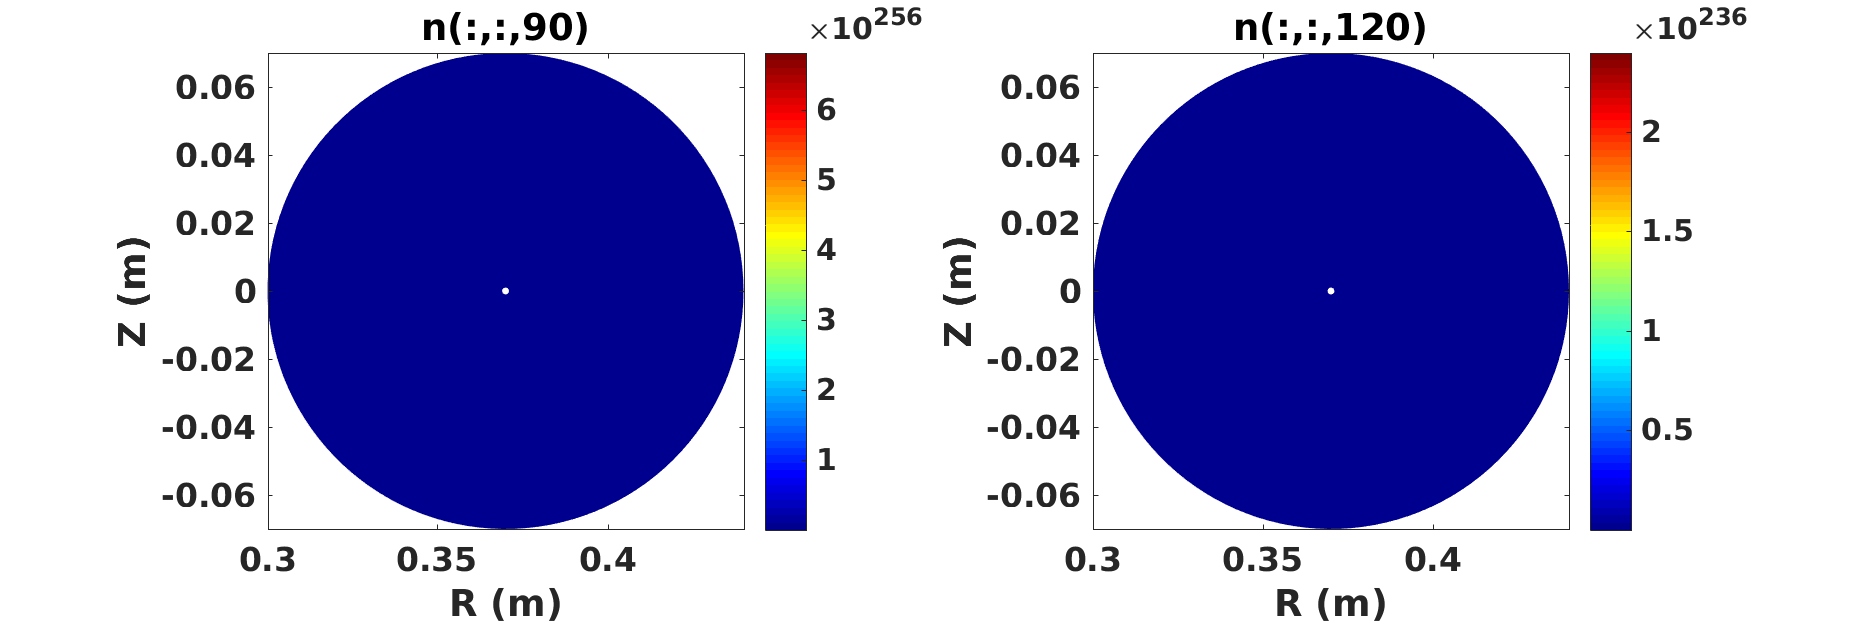
\includegraphics[scale=0.5]{../SImulacao_breakdown/Adaptacao_nova/ntod2.png} 
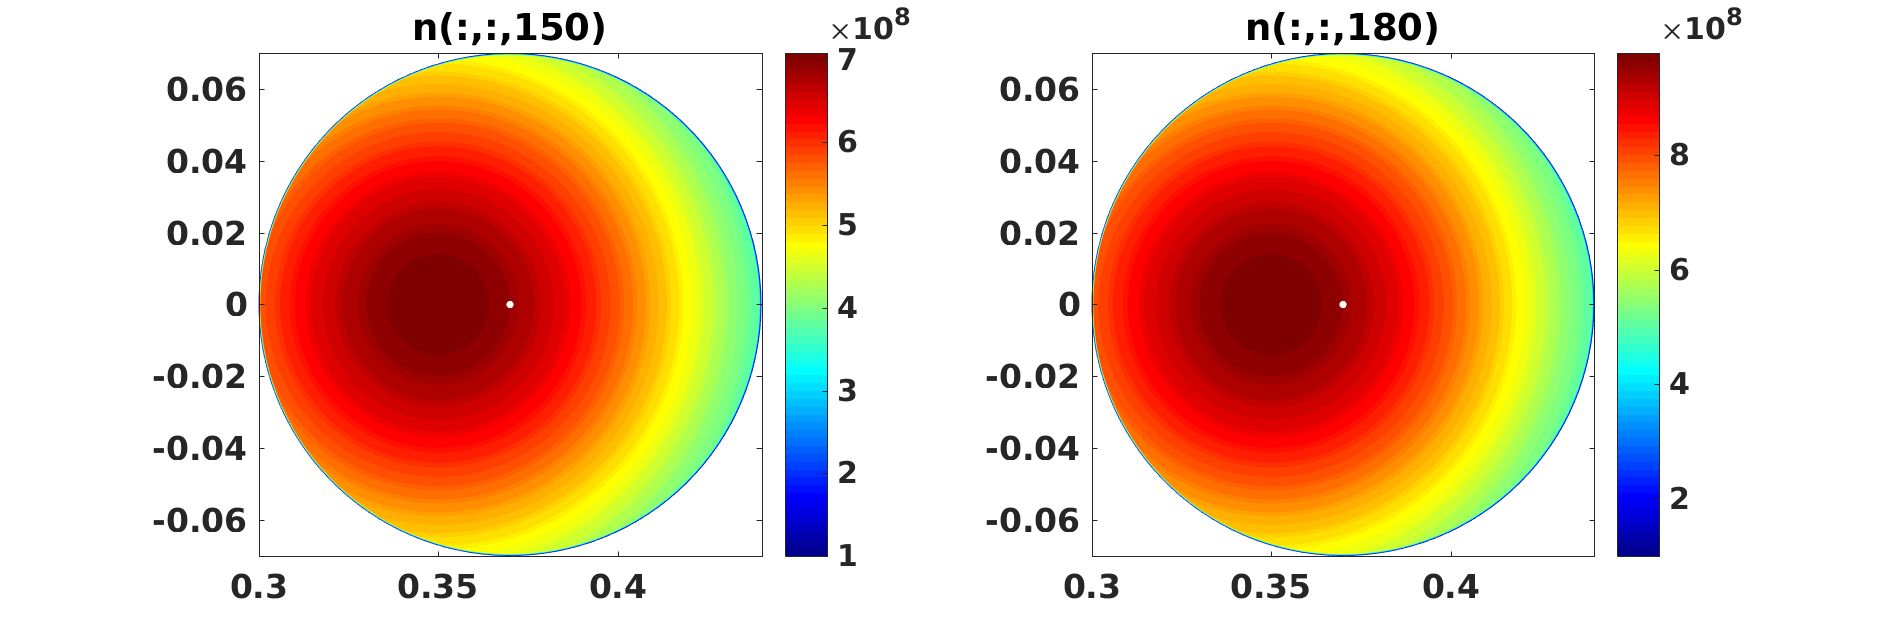
\includegraphics[scale=0.5]{../SImulacao_breakdown/Adaptacao_nova/ntod3.png} 
\caption{Resultado inicial, \textit{contourf} densidade numérica de partículas, $dt=10e-6$s, $Ng = 65$.}
\end{center}
\end{figure}

\begin{figure}[H]
\label{simul201}
\begin{center}
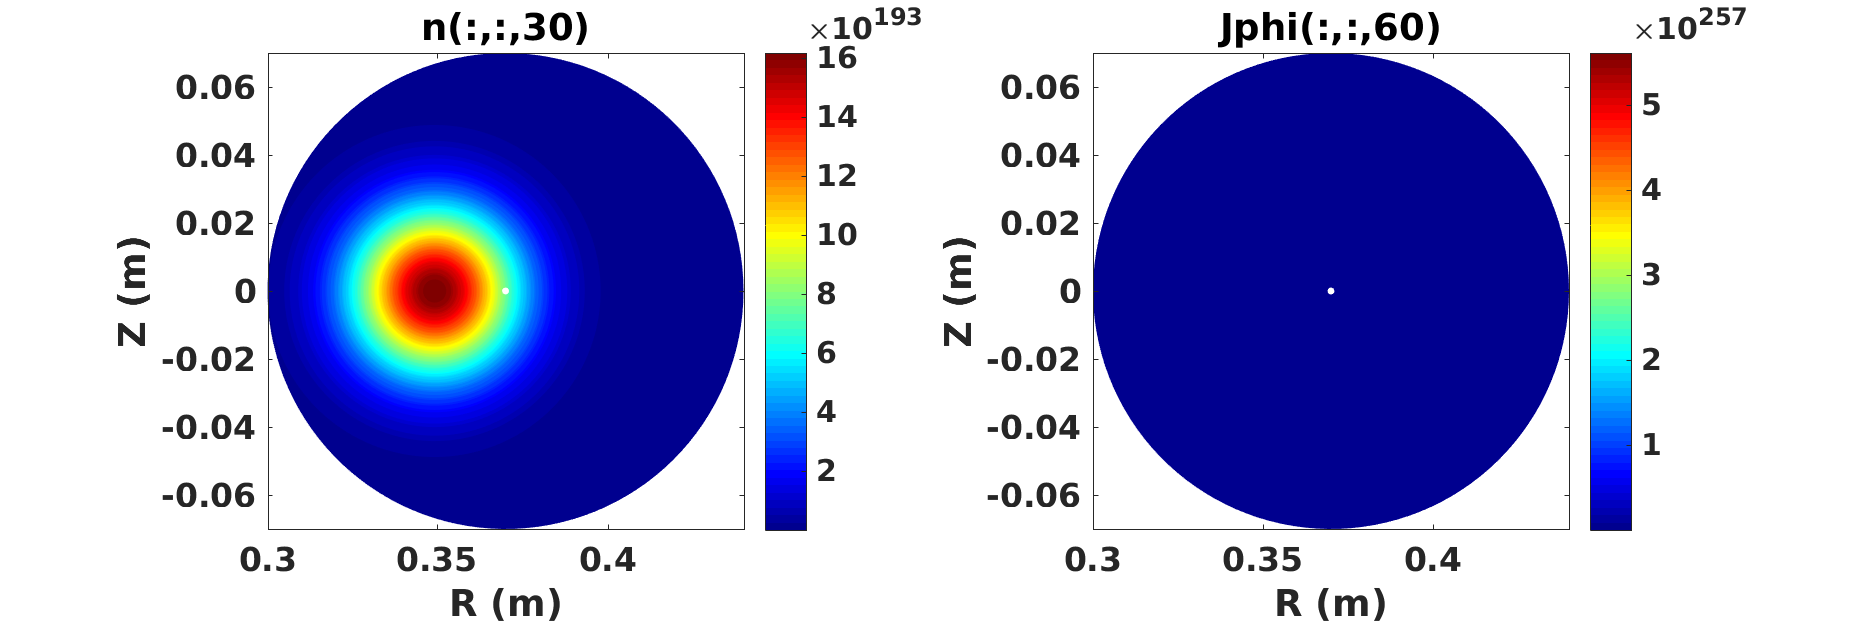
\includegraphics[scale=0.5]{../SImulacao_breakdown/Adaptacao_nova/jtod1.png}  
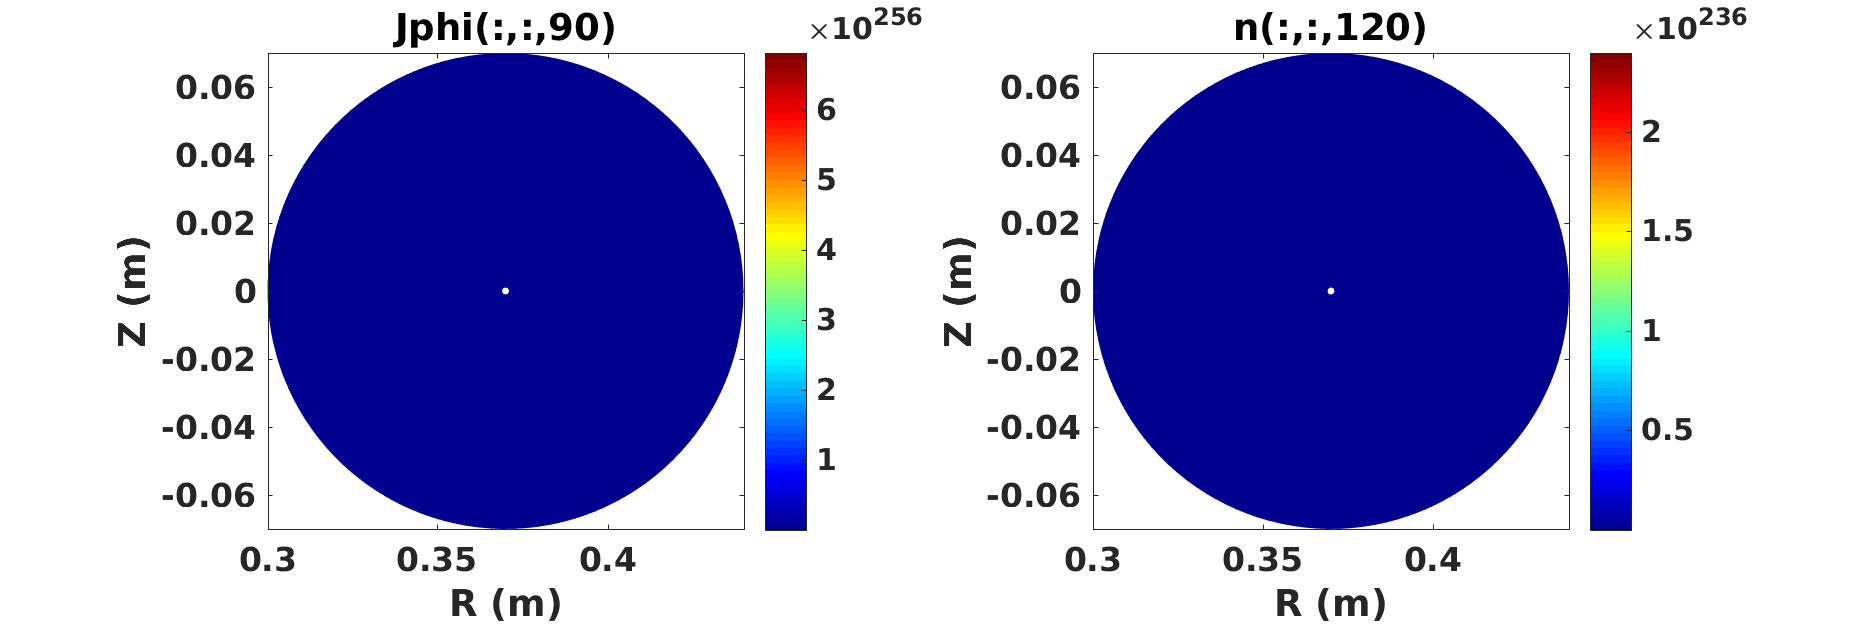
\includegraphics[scale=0.5]{../SImulacao_breakdown/Adaptacao_nova/jtod2.png} 
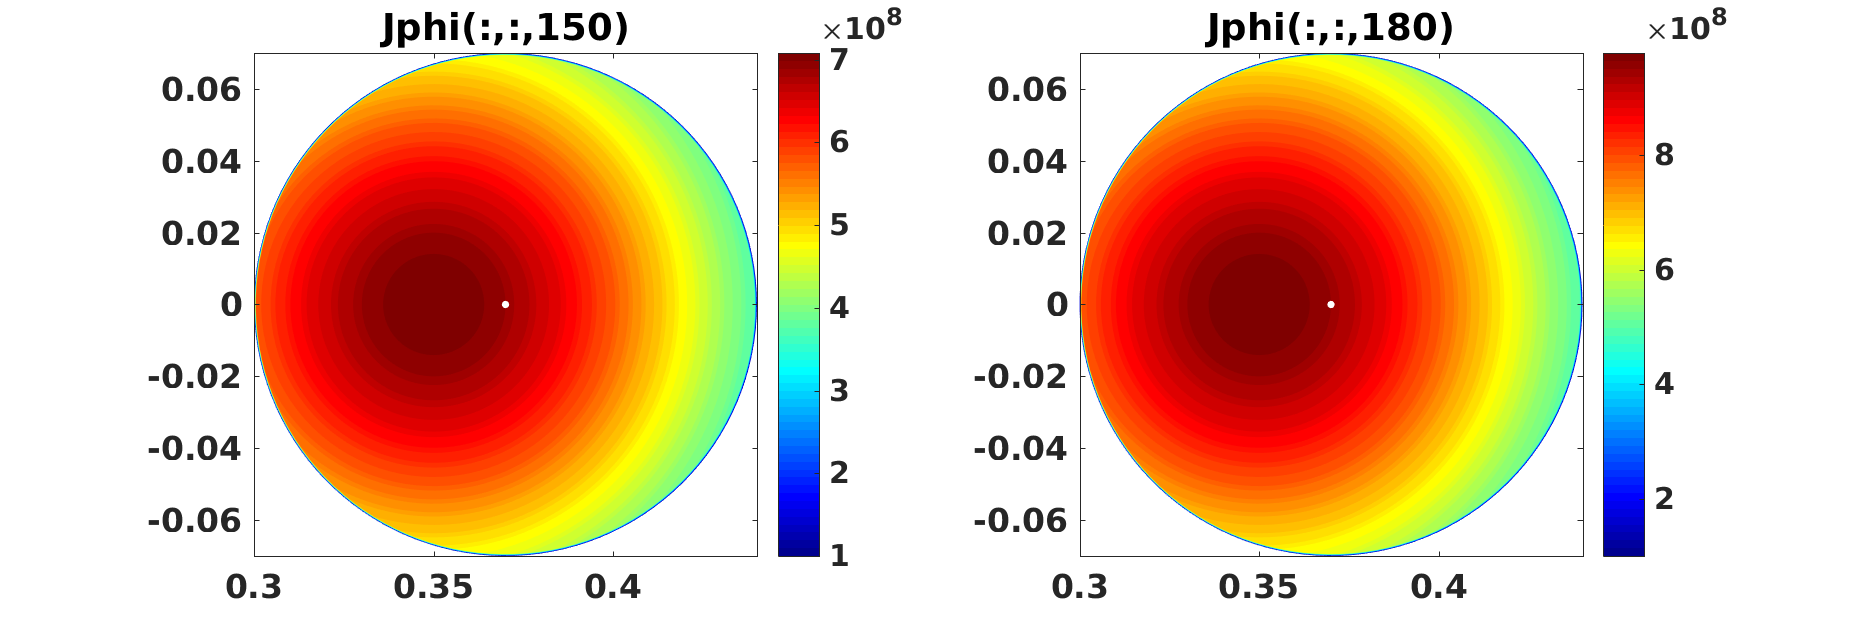
\includegraphics[scale=0.5]{../SImulacao_breakdown/Adaptacao_nova/jtod3.png} 
\caption{Resultado inicial, \textit{contourf} densidade de corrente na direção toroidal, $dt=10e-6$s, $Ng = 65$.}
\end{center}
\end{figure}
\begin{figure}[H]
\label{simul201}
\begin{center}
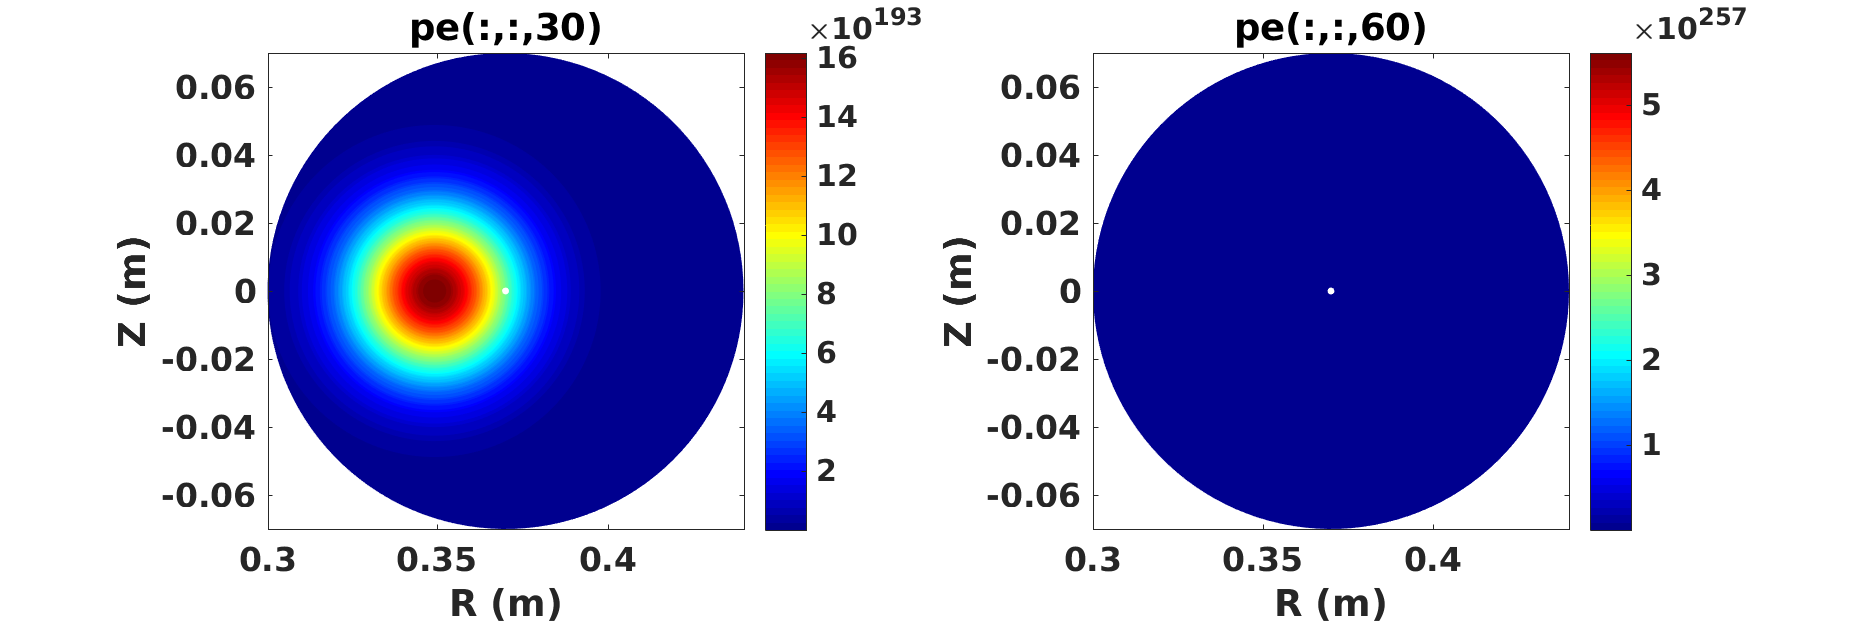
\includegraphics[scale=0.5]{../SImulacao_breakdown/Adaptacao_nova/petod1.png}  
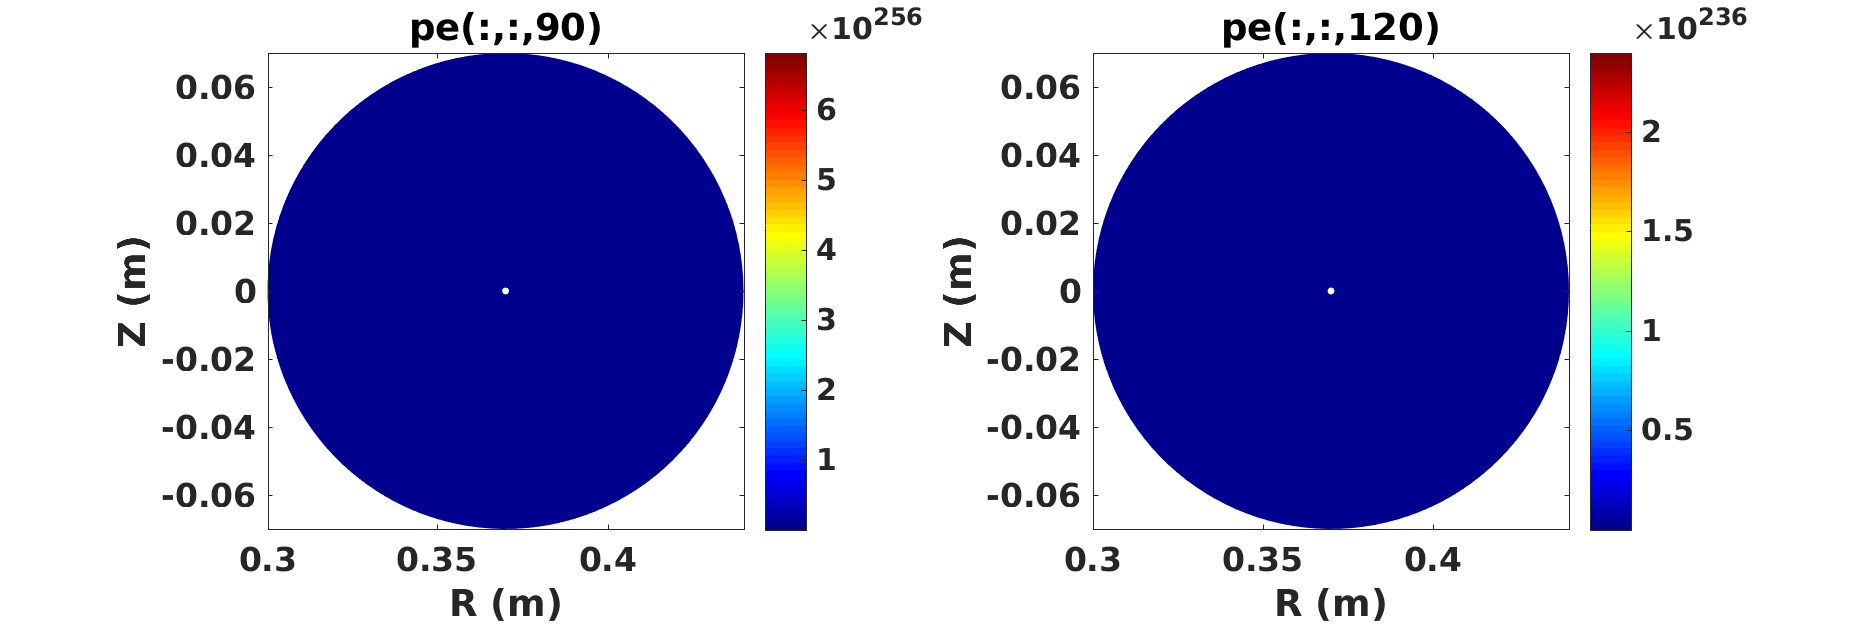
\includegraphics[scale=0.5]{../SImulacao_breakdown/Adaptacao_nova/petod2.png} 
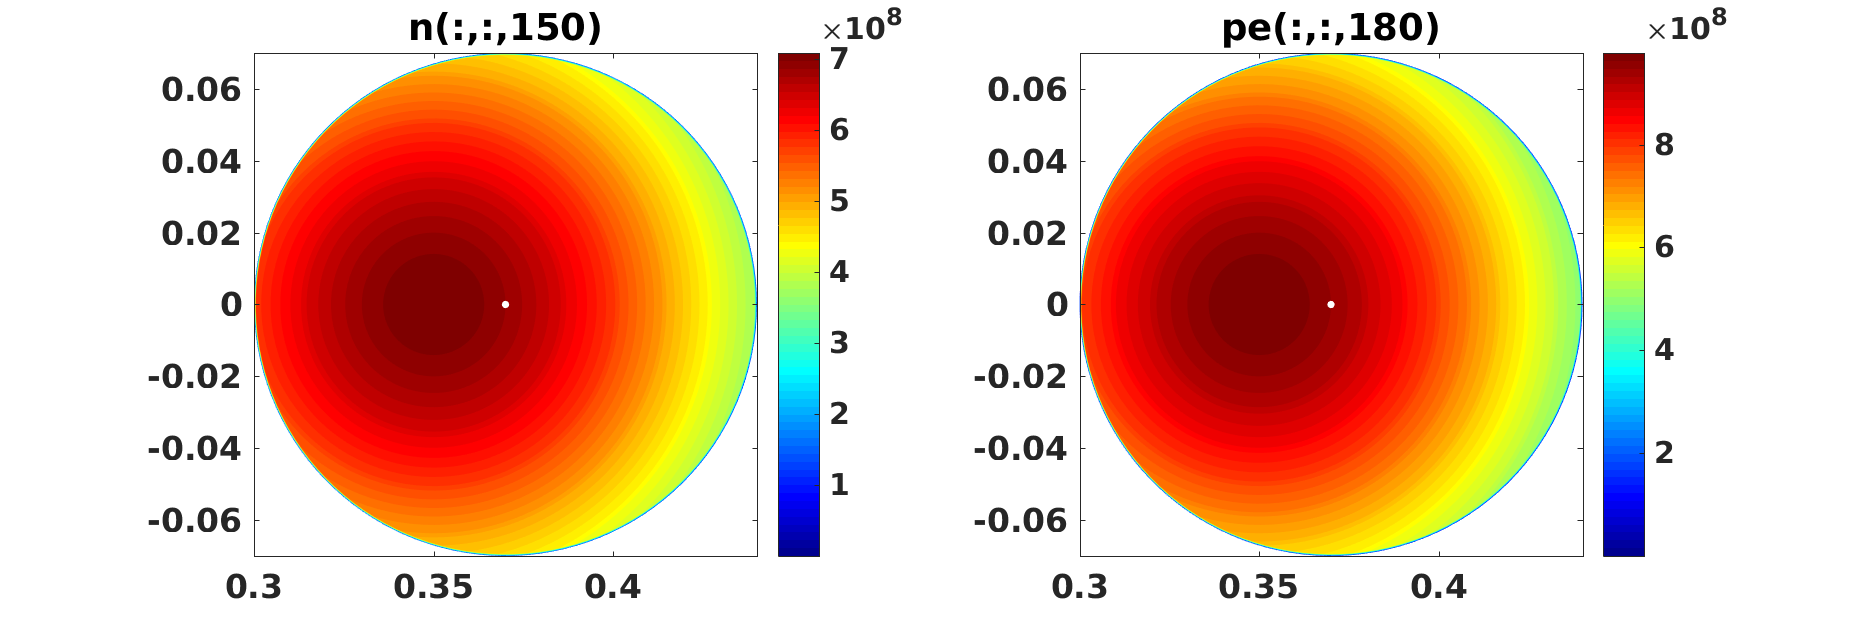
\includegraphics[scale=0.5]{../SImulacao_breakdown/Adaptacao_nova/petod3.png} 
\caption{Resultado inicial, \textit{contourf} pressões eletrônicas, $dt=10e-6$s, $Ng = 65$.}
\end{center}
\end{figure}
\begin{figure}[H]
\label{simul201}
\begin{center}
\includegraphics[scale=0.5]{../SImulacao_breakdown/Adaptacao_nova/pitod1.png}  
\includegraphics[scale=0.5]{../SImulacao_breakdown/Adaptacao_nova/pitod2.png} 
\includegraphics[scale=0.5]{../SImulacao_breakdown/Adaptacao_nova/pitod3.png} 
\caption{Resultado inicial, \textit{contourf} pressões iônicas, $dt=10e-6$s, $Ng = 65$.}
\end{center}
\end{figure}
\begin{comment}
\begin{figure}[H]
\label{simul0001}
\begin{center}
\includegraphics[scale=0.5]{../SImulacao_breakdown/Adaptacao_nova/Jphi(:,:,323).png}  
\caption{Resultado inicial, \textit{contourf} densidade numérica e densidade de corrente na direção toroidal, $dt=10e-5$s, $Ng = 65$.}
\end{center}
\end{figure}
\begin{figure}[H]
\label{simul14}
\begin{center}
\includegraphics[scale=0.5]{../SImulacao_breakdown/Adaptacao_nova/pion(:,:,323).png}  
\caption{Resultado inicial, \textit{contourf} pressões eletrônica e iônica, $dt=10e-6$s, $Ng = 65$.}
\end{center}
\end{figure}
\end{comment}
\begin{comment}
\begin{figure}[H]
\label{simul10}
\begin{center}
\includegraphics[scale=0.5]{../SImulacao_breakdown/Adaptacao_nova/Jphi(:,:,243).png}  
\caption{Resultado inicial, \textit{contourf} densidade numérica e densidade de corrente na direção toroidal, $dt=10e-5$s, $Ng = 65$.}
\end{center}
\end{figure}
\begin{figure}[H]
\label{simul11}
\begin{center}
\includegraphics[scale=0.5]{../SImulacao_breakdown/Adaptacao_nova/pion(:,:,243).png}  
\caption{Resultado inicial, \textit{contourf} pressões eletrônica e iônica, $dt=10e-6$s, $Ng = 65$.}
\end{center}
\end{figure}
\end{comment}

\begin{comment}
\begin{figure}[H]
\label{simul21}
\begin{center}
\includegraphics[scale=0.5]{../SImulacao_breakdown/Adaptacao_nova/Jphi(:,:,483).png}  
\caption{Resultado inicial, \textit{contourf} densidade numérica e densidade de corrente na direção toroidal, $dt=10e-5$s, $Ng = 65$.}
\end{center}
\end{figure}
\begin{figure}[H]
\label{simul22}
\begin{center}
\includegraphics[scale=0.5]{../SImulacao_breakdown/Adaptacao_nova/pion(:,:,483).png}  
\caption{Resultado inicial, \textit{contourf} pressões eletrônica e iônica, $dt=10e-6$s, $Ng = 65$.}
\end{center}
\end{figure}
\end{comment}
\end{comment}
